\documentclass[letterpaper,12pt,oneside]{article}
\usepackage[top=1in, left=1.25in, right=1.25in, bottom=1in]{geometry}
\usepackage[backend=bibtex, style=numeric]{biblatex}

\usepackage[T1]{fontenc}
\usepackage[utf8]{inputenc}
\usepackage[english]{babel}
\usepackage{caption, subcaption} %figuras
\usepackage{graphicx}
\usepackage{array}
\usepackage{amsmath} 
\usepackage{amssymb} 
\usepackage{tikz}
\usepackage{imakeidx}
\usepackage{biblatex}
\addbibresource{bib/protocolo.bib}
\usepackage{float}
\usepackage{verbatim}

\graphicspath{{./figs/}}
\usepackage{setspace}
%\usepackage[round]{natbib}
\allowdisplaybreaks
\begin{document}
%\frontmatter
\begin{titlepage}
		\setlength{\parindent}{0pt} \setlength{\parskip}{0pt}
	
		\begin{center}
			\vfill 
			
			\begin{minipage}{\textwidth}
				
				\newcolumntype{V}{>{\centering\arraybackslash} m{.17\textwidth} }
				\newcolumntype{C}{>{\centering\arraybackslash} m{.56\textwidth} }
				
				\begin{center}
					
\includegraphics[width=4.5cm]{UNAM_LOGO2.png}	
				\end{center} 	
				\begin{center}
					\Huge\textbf{Universidad Nacional Autónoma de México}
				\end{center} 
				
			\end{minipage}
				
			\vfill
			
			\begin{minipage}{0.7\textwidth}
				\begin{center}
					\large Ingeniería en Computación
				\end{center}
			\end{minipage}
			% 
			\begin{center}
				%\medskip \rule{.9\textwidth}{2pt}
				\vfill
				\large Compilers
				%{\Large \bfseries  \title   }
				
				%\medskip \rule{.9\textwidth}{2pt}
			\end{center}
			
			\begin{center}
				\vspace*{1cm}
				{\huge Compiler}\\
				\vspace*{1cm}
				
				%PRESENTA:\\ \medskip
				\begin{center}
					STUDENTS: \\
					\large 321184995\\
                    \large 321331656\\
                    \large 321058526\\
                    \large 424138220\\
                    \large 320560154
				\end{center}
				
				\bigskip
				
				Group: \\
				\#05\\
				%Coadvisors
				Semester: \\
                2026-II
			\end{center}
			
			\vfill
			
			\begin{center}
				{Mexico, CDMX. 28th May 2026}\\
			\end{center}
			\cleardoublepage
		\end{center}
	\end{titlepage}
 
\tableofcontents
\clearpage
    
%\mainmatter

\section{Introduction} %
\begin{comment}
Este apartado debe abordar los siguientes puntos:
\begin{itemize}
    \item \textbf{Planteamiento del problema.} Se hace una descripción del problema a resolver.
    \item \textbf{Motivación.} Se describe porqué es necesario dar solución al problema.
    \item \textbf{Objetivos.} Lo que se se espera obtener de darle solución al problema.
\end{itemize}
\end{comment}
    Compilers are fundamental tools in software development and computer programming because they allow the transformation of high-level source code into low-level instructions that can be directly executed by the processor. However, this process does not simply consist of translating text; it requires a sequence of stages responsible for analyzing, validating, and transforming the source code into an executable representation.
    \\ \\ 
    The compilation process is divided into several phases: lexical analysis, syntax analysis, semantic analysis, intermediate code generation, code optimization, and target code generation. Each stage fulfills a specific function and depends on the correct execution of the previous phase. In particular, lexical analysis represents the first phase of the compiler and is responsible for examining source code and dividing it into basic units called tokens. These tokens correspond to meaningful language elements such as reserved words, identifiers, constants, operators, and punctuation symbols.
    \\ \\
    However, identifying valid tokens is not sufficient to guarantee that a program is correctly constructed. Once the token sequence is obtained, it is necessary to verify that these tokens follow the grammatical structure defined for the programming language and that they also possess logical and semantic consistency. For this purpose, syntax analysis through a Parser and the application of Syntax Directed Translation (SDT) techniques are required to validate essential semantic rules such as type compatibility, valid variable declarations, and the proper construction of expressions and assignments.
    \\ \\ 
    The problem addressed in this project consists of the design and implementation of a compiler focused on processing .c source code files. The system must be capable of receiving programs written in the C programming language, performing lexical analysis to separate and classify lexemes, validating the syntactic structure through a Parser, and applying semantic rules using SDT. In this way, the compiler will be able to detect errors during the earliest phases of the compilation process and build a structured representation of the program.
    \\ \\
    Without tools such as the lexer, parser, and semantic analyzer, the compilation process would be incapable of understanding the intention behind the programmer’s code, limiting itself to interpreting characters without structural meaning. Therefore, these stages constitute the fundamental basis that allows a sequence of text to be transformed into a logical and meaningful representation understandable by the system.
    \\ \\
    The system must follow a structured processing flow. First, the compiler receives a set of instructions contained in a C source code file. Subsequently, the input strings are processed through different analyzers, beginning with lexical analysis, followed by syntax and semantic analysis, in order to validate both the grammatical structure and the logical consistency of the program. Finally, once these stages are completed, the system generates a valid representation of the code that can be linked and prepared for execution, displaying the corresponding results of the compilation process.
    \\ \\
    Understanding the internal mechanics of a compiler is a fundamental pillar in software systems development, as it reveals the exact processes through which a computer processes, interprets, and validates a programming language.
    \\ \\
    The primary motivation behind this project lies in breaking down and resolving the complexities of error detection prior to program execution. Lexical analysis, acting as the first line of defense, holds critical relevance: it not only streamlines the input stream by stripping away irrelevant elements like comments and whitespace, but it also establishes a clean structure of tokens that is indispensable for the success of subsequent phases.
    \\ \\
    Furthermore, constructing a parser and integrating a Syntax-Directed Translation (SDT) scheme allows high-abstraction concepts, such as context-free grammars, LR automata, ACTION/GOTO tables, and shift-reduce algorithms, to materialize into a fully functional software architecture. This hands-on implementation provides firsthand experience in how a system simultaneously validates both the grammatical structure and the logical coherence of a program.
    \noindent\subsection*{General Objective:}
    Design and implement a compiler capable of processing source code files written in C language. The system will perform lexical, syntactic, and semantic analyses to validate the grammatical structure, logical coherence, and correct construction of the input program.
    \noindent\subsection*{Specific Objectives:}
    \begin{itemize}
        \item Develop a lexical analyzer to identify and classify source code components into specific tokens, such as keywords, identifiers, operators, constants, and punctuation marks, while filtering out irrelevant elements like whitespace and comments.
        \item Design an efficient parser to validate the grammatical structure of the C language subset utilizing syntactic analysis techniques.
        \item Implement a Syntax-Directed Translation (SDT) scheme to perform type checking, variable declaration verification, and other essential semantic validations concurrently with the parsing process.
        \item Detect lexical, syntactic, and semantic errors present in the source code.
        \item Build auxiliary structures such as symbol tables and hierarchical representations of the program.
    \end{itemize}

\section{Theoretical Framework}
\begin{comment}
Son los conceptos aplicados, principalmente los vistos en clase, con los que se va a dar solución al problema, explicados de forma concreta, ya sea con su interpretación personal o bien con referencias bibliográficas sólidas.~\cite{10.5555/576122}
\end{comment}
    \subsection{Compilers}
    A programming language is defined as a set of rules and notations that allow us to communicate with computers in order to develop software, applications, and systems. However, for a program to be executed, it is necessary to translate it into a format that the computer can understand and execute. The systems responsible for this process are known as compilers.
    \\ \\
    The compiler transforms high-level source code into low-level target code that the processor can execute directly. In general, this process can be understood as two blocks that perform different activities: analysis and synthesis.
    \\ \\
    In the analysis phase, the compiler acts as a "critical reader," whose objective is to understand the source code and verify that it is correct. It is divided into lexical analysis, syntax analysis, and semantic analysis. At the end of this phase, an intermediate representation is generated, which is a version of the code that is no longer text, but is still not machine language.
    \\ \\
    In the synthesis phase, the compiler is responsible for efficiency and the technical construction of the executable. It takes the validated intermediate representation and translates it into the target language. It mainly consists of intermediate code generation, code optimization, and target code generation.\cite{aho2008compiladores}
    \\ \\
    Compiler is divided into six phases: lexical analyzer, syntactic analyzer, semantic analyzer, intermediate code generation, code optimization, and target code generation.

    \subsection{Lexical Analysis}
    The first phase of compilation is called lexical analysis. In this phase, the analyzer takes the source code as input, reads its characters, and groups them into meaningful units called tokens, together with a terminal symbol used to make syntax analysis decisions. A token represents a lexical category within a programming language, such as:
    \begin{itemize}
        \item Keywords (int, float, return)
        \item Identifiers (x, a, b, c)
        \item Operators (=, +, -, *)
        \item Constants (2, 3, 5, 0)
        \item Punctuation marks ((, ), \{, \}, ;)
        \item Literal ("Hello World")
    \end{itemize}
     An input sequence that forms a token is called a lexeme; therefore, the lexical analyzer isolates the syntax analyzer from token representation through lexemes. To perform this recognition, lexical analyzers use pattern identification mechanisms that allow each fragment of the input text to be classified. These patterns are generally described through regular expressions, which formally define how certain language elements can be formed.\cite{aho2008compiladores}

    \subsection{Context Free Grammar (CFG)}
    Once the token sequence has been obtained, the syntax analysis phase begins. However, before explaining this process, it is necessary to understand Context-Free Grammars (CFG), since they are the formal basis of syntax analysis. In general, a grammar can be defined using the quadruple:
    \begin{center}
        G = (V, $\Sigma$, P, S)
    \end{center}
    Where:
    \begin{itemize}
        \item V - syntactic variables that denote sets of strings, known as non-terminals. The sets of strings denoted by non-terminals help define the language generated by the grammar. Non-terminals impose a hierarchical structure on the language, making them key for syntax analysis.
        \item $\Sigma$ - basic symbols from which strings are formed, known as terminals. Terminals are the primary components of the tokens produced by the lexical analyzer.
        \item P - refers to the productions of a grammar. These specify how terminals and non-terminals can be combined to form strings.
        \item S - represents the start symbol. This symbol is a special non-terminal from which the derivation of strings in the language defined by the grammar begins.
    \end{itemize}
    CFGs help us specify the syntax of a programming language; each language has precise rules that prescribe the syntactic structure of well-formed programs. However, these rules constitute only a theoretical model. The transition to the implementation phase occurs when the syntax analyzer assumes the operational role.\cite{aho2008compiladores}
    
    \subsection{Syntax Analysis (Parser)}
    The syntax analyzer (Parser), once the token sequence is ready, is responsible for verifying that the sequence of token names can be generated by the grammar of the source language. The syntax analyzer organizes tokens into syntactic classes, also called non-terminals in the grammar, such as expressions, procedures, and other elements. If the sequence respects the established production rules, then it is considered syntactically valid, and the result is a parse tree, where the leaves represent the tokens and the internal nodes correspond to the syntactic classes, showing how the program structure is organized according to the grammar. Otherwise, the compiler reports a syntax error.\cite{aho2008compiladores}
    \\ \\
    The general process of syntax analysis can be represented in the following phases:
    \begin{itemize}
        \item Token Reception: The lexical analyzer delivers the token sequence to the syntax analyzer.
        \item Verification: It checks whether the tokens match the grammar production rules.
        \item Parse Tree Construction: It represents the hierarchical structure of the program according to the grammatical rules.
        \item Error Generation: If it finds an invalid sequence, it generates an error message indicating the problem.
    \end{itemize}

    \subsection{Parsing Methods}
    Parsing methods are classified into:
    \begin{itemize}
        \item Top-Down: This method derives the input starting from the start symbol and expanding productions until matching the received tokens; that is, it builds parse trees from the top (root) to the bottom (leaves). This same classification is divided into non-deterministic and deterministic methods. Non-deterministic parsers are those that, when facing a decision, do not know with certainty which path to take and must try alternatives (brute force). Deterministic parsers are those that can predict exactly which rule to use, based only on the current symbol. Among deterministic parsers are LL(1) parsers, which use one lookahead symbol to decide which production to apply. Top-Down syntax analysis is usually easier to implement manually, although it requires eliminating ambiguity, left recursion, and applying factoring when necessary.\cite{aho2008compiladores}
        \item Bottom-Up: This method works in the opposite way to Top-Down methods: it begins with the input tokens and attempts to reduce sequences until reaching the start symbol; that is, it builds parse trees from the leaves upward to the root. As with the previous method, Bottom-Up parsers can be classified as ambiguous and predictive. Ambiguous parsers may explore multiple reduction paths simultaneously in the presence of ambiguity. Predictive parsers use lookahead symbols to make deterministic decisions without needing backtracking; these include LR, SLR, LALR, and CLR parsers.\\
        These parsers are more powerful than Top-Down parsers, since they accept a wider variety of grammars and are widely used in automatic tools such as Yacc or Bison.\cite{aho2008compiladores}
    \end{itemize}

    \subsection{FIRST Sets}
    FIRST sets determine which terminals may appear at the beginning of derivations. \\
    Formally:
    \begin{center}
        FIRST($\alpha$)
    \end{center}
    represents the set of terminal symbols that can start derived strings from $\alpha$. \\ \\
    These sets are essential for:
    \begin{itemize}
        \item Calculating lookaheads.
        \item Constructing LR items
        \item Generating parsing tables.
    \end{itemize}

    \subsection{LR(1) Items and Closure}
    An \textbf{LR(1) item} is a production with a dot ($\bullet$) indicating how much we have parsed, plus a lookahead terminal. Example:
	
	\[
	E \rightarrow E \; \bullet \; + \; T \quad , \quad \text{lookahead} = \{ \$, +, ) \}
	\]
    The Closure operation automatically expands elements when the period appears before a non-terminal, adding new productions needed to continue the syntactic analysis.\cite{gfg_sdt_2025}

    \subsection{GOTO and State Construction}
    The GOTO function allows shifting the dot over a symbol and constructing new states of the LR automaton.
    \\ \\ 
    Formally:
    \[
	\text{goto}(I, X) = \text{closure}(\{ A \rightarrow \alpha X \bullet \beta , a \mid A \rightarrow \alpha \bullet X \beta , a \in I \})
	\]
    State construction is fundamental for generating the ACTION and GOTO tables used during parsing.\cite{gfg_sdt_2025}
    
    \subsection{Shift-Reduce Parsing}
    Shift-Reduce parsing simulates an LR automaton using stacks. \\
    The main operations are:
    \begin{itemize}
        \item \textbf{Shift}: Shifts a token onto the stack.
        \item \textbf{Reduce}: Applies a grammar production.
        \item \textbf{Accept}: Indicates that the input is valid.
        \item \textbf{Error}: Indicates an invalid sequence.
    \end{itemize}
    The parser uses:
    \begin{itemize}
        \item A state stack
        \item A semantic stack for SDT (Syntax-Directed Translation).
    \end{itemize}

    \subsection{Syntax-Directed Translation}
    Syntax-Directed Translation (SDT) allows executing semantic actions during the parsing process. \\
    Each grammar production has associated actions that allow:
    \begin{itemize}
        \item Constructing abstract syntax trees,
        \item Checking types,
        \item Managing symbol tables,
        \item Evaluating expressions,
        \item Detecting semantic errors.
    \end{itemize}
    SDT uses semantic attributes: \\ \\
    \textbf{Synthesized attributes} \\
    They flow from the children to the parent node. \\ \\
    \textbf{Inherited attributes} \\
    They receive information from the parent or siblings. 

    \subsection{Abstract Syntax Tree (AST)}
    The Abstract Syntax Tree (AST) represents the logical structure of the program, eliminating unnecessary elements such as parentheses or delimiters.\cite{gfg_sdt_2025} \\ 
    The nodes implemented in the project include:
    \begin{itemize}
        \item Constants 
        \item Identifiers
        \item Arithmetic operators
        \item Declarations
    \end{itemize}
    The AST facilitates the subsequent stages of validation and code generation.

    \subsection{Symbol Table}
    The symbol table stores information related to variables and program elements. \\
    Among the stored data are:
    \begin{itemize}
        \item Name 
        \item Type
        \item Value
        \item Scope
    \end{itemize}
    The table allows:
    \begin{itemize}
        \item Registering variables 
        \item Verifying declarations
        \item Validating usages,
        \item Detecting redeclarations
    \end{itemize}

    \subsection{Intermediate Code Generation}
    After the source code has been lexically, syntactically, and semantically validated, many compilers generate an intermediate representation of the program before producing machine code. This intermediate representation decouples the analysis and synthesis phases of the compiler, facilitating optimization and portability between architectures. \\ \\
    The generation of intermediate code simplifies subsequent stages such as optimization and target code generation, as it provides a representation that is easier to manipulate than the original source code.

    \subsection{Code Optimization}
    Code optimization is the phase responsible for improving the program's efficiency without altering its logical behavior. Its primary goal is to reduce execution time, memory consumption, or the size of the generated code. \\
    Optimizations can be classified into:
    \begin{itemize}
        \item Machine-independent optimizations
        \item Machine-dependent optimizations
    \end{itemize}
    Among the most common techniques are:
    \begin{itemize}
        \item Dead code elimination
        \item Constant propagation
        \item Algebraic simplification
        \item Common sub expression elimination
        \item Loop optimization
    \end{itemize}

    \subsection{Target Code Generation}
    Target code generation constitutes the final phase of the compiler. Its purpose is to translate the intermediate representation into specific instructions for a hardware architecture. \\
    The target code can produce:
    \begin{itemize}
        \item Assembly code
        \item Machine code
        \item Bytecode
        \item Object files
    \end{itemize}
    During this phase, the compiler must consider aspects such as:
    \begin{itemize}
        \item Register management,
        \item Memory addressing,
        \item CPU instructions,
        \item Handling function calls.
    \end{itemize}
    Target code generation allows the program to execute directly on the target system.
    \subsection{Linker and Execution}
    After generating the target code, the linker comes into play. Its function consists of combining different object files, libraries, and external references to produce a final executable. \\
    The linker resolves:
    \begin{itemize}
        \item Function references
        \item Global variables
        \item Memory addresses
        \item External dependencies
    \end{itemize}
    Once the linking is completed, the system generates an executable program capable of running directly on the corresponding operating system and processor.\\
    Within the compiler's general workflow, this stage represents the final transition between source code analysis and the actual execution of the program.







    

    


\section{Development}

\subsection{Grammar}
\begin{align*}
\text{Program'} &\rightarrow \text{Program} \\
\text{Program} &\rightarrow \text{TopLevelList} \\
\text{TopLevelList} &\rightarrow \text{TopLevel} \mid \text{TopLevelList} \quad \text{TopLevel} \\
\text{TopLevel} &\rightarrow \text{Statement} \mid \text{FunctionDecl} \\
\\
\text{StatementList} &\rightarrow \text{Statement} \mid \text{StatementList} \quad \text{Statement} \\
\text{Statement} &\rightarrow \text{Declaration} \quad \texttt{;} \mid \text{Assignment} \quad \texttt{;} \mid \text{Block} \\
\text{Declaration} &\rightarrow \text{TYPE} \quad \text{DeclList} \\
\text{DeclList} &\rightarrow \text{DeclItem} \mid \text{DeclList} \quad \texttt{,} \quad \text{DeclItem} \\
\text{DeclItem} &\rightarrow \text{ID} \\
                &\mathrel{\phantom{\rightarrow}} \mid \text{ID} \quad \texttt{=} \quad \text{E} \\
                &\mathrel{\phantom{\rightarrow}} \mid \text{ID} \quad \texttt{[} \quad \text{E} \quad \texttt{]} \\
                &\mathrel{\phantom{\rightarrow}} \mid \text{ID} \quad \texttt{[} \quad \text{E} \quad \texttt{]} \quad \texttt{=} \quad \texttt{\{} \quad \text{InitList} \quad \texttt{\}} \\
                &\mathrel{\phantom{\rightarrow}} \mid \text{ID} \quad \texttt{[} \quad \text{E} \quad \texttt{]} \quad \texttt{[} \quad \text{E} \quad \texttt{]} \\
                &\mathrel{\phantom{\rightarrow}} \mid \text{ID} \quad \texttt{[} \quad \text{E} \quad \texttt{]} \quad \texttt{[} \quad \text{E} \quad \texttt{]} \quad \texttt{=} \quad \texttt{\{} \quad \text{MatrixInitList} \quad \texttt{\}} \\
\text{Assignment} &\rightarrow \text{ID} \quad \texttt{=} \quad \text{E} \\
                  &\mathrel{\phantom{\rightarrow}} \mid \text{ArrayAccess} \quad \texttt{=} \quad \text{E} \\
                  &\mathrel{\phantom{\rightarrow}} \mid \text{MatrixAccess} \quad \texttt{=} \quad \text{E} \\
\text{Block} &\rightarrow \texttt{\{} \quad \text{StatementList} \quad \texttt{\}} \mid \texttt{\{} \quad \texttt{\}} \\
\\
\text{E} &\rightarrow \text{OrExpr} \\
\text{OrExpr} &\rightarrow \text{OrExpr} \quad \texttt{||} \quad \text{AndExpr} \mid \text{AndExpr} \\
\text{AndExpr} &\rightarrow \text{AndExpr} \quad \texttt{\&\&} \quad \text{EqExpr} \mid \text{EqExpr} \\
\text{EqExpr} &\rightarrow \text{EqExpr} \quad \texttt{==} \quad \text{RelExpr} \mid \text{EqExpr} \quad \texttt{!=} \quad \text{RelExpr} \mid \text{RelExpr} \\
\text{RelExpr} &\rightarrow \text{RelExpr} \quad \texttt{<} \quad \text{AddExpr} \\
               &\mathrel{\phantom{\rightarrow}} \mid \text{RelExpr} \quad \texttt{>} \quad \text{AddExpr} \\
               &\mathrel{\phantom{\rightarrow}} \mid \text{RelExpr} \quad \texttt{<=} \quad \text{AddExpr} \\
               &\mathrel{\phantom{\rightarrow}} \mid \text{RelExpr} \quad \texttt{>=} \quad \text{AddExpr} \\
               &\mathrel{\phantom{\rightarrow}} \mid \text{AddExpr} \\
\text{AddExpr} &\rightarrow \text{AddExpr} \quad \texttt{+} \quad \text{MulExpr} \mid \text{AddExpr} \quad \texttt{-} \quad \text{MulExpr} \mid \text{MulExpr} \\
\text{MulExpr} &\rightarrow \text{MulExpr} \quad \texttt{*} \quad \text{UnaryExpr} \\
               &\mathrel{\phantom{\rightarrow}} \mid \text{MulExpr} \quad \texttt{/} \quad \text{UnaryExpr} \\
               &\mathrel{\phantom{\rightarrow}} \mid \text{MulExpr} \quad \texttt{\%} \quad \text{UnaryExpr} \\
               &\mathrel{\phantom{\rightarrow}} \mid \text{UnaryExpr} \\
\text{UnaryExpr} &\rightarrow \texttt{!} \quad \text{UnaryExpr} \mid \texttt{-} \quad \text{UnaryExpr} \mid \texttt{+} \quad \text{UnaryExpr} \mid \text{Primary} \\
\text{Primary} &\rightarrow \texttt{(} \quad \text{E} \quad \texttt{)} \mid \text{ID} \mid \text{CONST} \mid \text{FunctionCall} \mid \text{ArrayAccess} \mid \text{MatrixAccess} \\
\text{Statement} &\rightarrow \text{IfStatement} \\
\text{IfStatement} &\rightarrow \texttt{if} \quad \texttt{(} \quad \text{E} \quad \texttt{)} \quad \text{Block} \mid \texttt{if} \quad \texttt{(} \quad \text{E} \quad \texttt{)} \quad \text{Block} \quad \texttt{else} \quad \text{Block} \\
\text{Statement} &\rightarrow \text{WhileStatement} \\
\text{WhileStatement} &\rightarrow \texttt{while} \quad \texttt{(} \quad \text{E} \quad \texttt{)} \quad \text{EnterBreak} \quad \text{EnterLoop} \quad \text{Block} \quad \text{ExitLoop} \quad \text{ExitBreak} \\
\text{Statement} &\rightarrow \text{ForStatement} \\
\text{ForStatement} &\rightarrow \texttt{for} \quad \texttt{(} \quad \text{ForInit} \quad \texttt{;} \quad \text{E} \quad \texttt{;} \quad \text{ForUpdate} \quad \texttt{)} \\
                    &\mathrel{\phantom{\rightarrow}} \quad \text{EnterBreak} \quad \text{EnterLoop} \quad \text{Block} \quad \text{ExitLoop} \quad \text{ExitBreak} \\
\text{ForInit} &\rightarrow \text{ID} \quad \texttt{=} \quad \text{E} \mid \text{Declaration} \\
\text{ForUpdate} &\rightarrow \text{ID} \quad \texttt{=} \quad \text{E} \mid \text{ID} \quad \texttt{++} \mid \text{ID} \quad \texttt{--} \\
\text{Statement} &\rightarrow \text{SwitchStatement} \\
\text{SwitchStatement} &\rightarrow \texttt{switch} \quad \texttt{(} \quad \text{E} \quad \texttt{)} \quad \texttt{\{} \quad \text{EnterBreak} \quad \text{CaseList} \quad \texttt{\}} \quad \text{ExitBreak} \\
                       &\mathrel{\phantom{\rightarrow}} \mid \texttt{switch} \quad \texttt{(} \quad \text{E} \quad \texttt{)} \quad \texttt{\{} \quad \text{EnterBreak} \quad \text{CaseList} \\
                       &\mathrel{\phantom{\rightarrow}} \quad \text{DefaultItem} \quad \texttt{\}} \quad \text{ExitBreak} \\
                       &\mathrel{\phantom{\rightarrow}} \mid \texttt{switch} \quad \texttt{(} \quad \text{E} \quad \texttt{)} \quad \texttt{\{} \quad \text{EnterBreak} \quad \text{DefaultItem} \\
                       &\mathrel{\phantom{\rightarrow}} \quad \texttt{\}} \quad \text{ExitBreak} \\
\text{CaseList} &\rightarrow \text{CaseItem} \mid \text{CaseList} \quad \text{CaseItem} \\
\text{CaseItem} &\rightarrow \texttt{case} \quad \text{CONST} \quad \texttt{:} \quad \text{Block} \\
\text{DefaultItem} &\rightarrow \texttt{default} \quad \texttt{:} \quad \text{Block} \\
\text{Statement} &\rightarrow \text{BreakStatement} \quad \texttt{;} \\
\text{BreakStatement} &\rightarrow \texttt{break} \\
\text{EnterBreak} &\rightarrow \epsilon \\
\text{ExitBreak} &\rightarrow \epsilon \\
\text{Statement} &\rightarrow \text{ContinueStatement} \quad \texttt{;} \\
\text{ContinueStatement} &\rightarrow \texttt{continue} \\
\text{EnterLoop} &\rightarrow \epsilon \\
\text{ExitLoop} &\rightarrow \epsilon \\
\text{FunctionDecl} &\rightarrow \text{FunctionHeader} \quad \text{EnterFunction} \quad \text{FunctionBody} \quad \text{ExitFunction} \\
\text{FunctionHeader} &\rightarrow \text{TYPE} \quad \text{ID} \quad \texttt{(} \quad \texttt{)} \mid \text{TYPE} \quad \text{ID} \quad \texttt{(} \quad \text{ParamList} \quad \texttt{)} \\
\text{ParamList} &\rightarrow \text{Param} \mid \text{ParamList} \quad \texttt{,} \quad \text{Param} \\
\text{Param} &\rightarrow \text{TYPE} \quad \text{ID} \\
\text{FunctionBody} &\rightarrow \texttt{\{} \quad \text{EnterParams} \quad \text{StatementList} \quad \texttt{\}} \mid \texttt{\{} \quad \text{EnterParams} \quad \texttt{\}} \\
\text{EnterFunction} &\rightarrow \epsilon \\
\text{ExitFunction} &\rightarrow \epsilon \\
\text{EnterParams} &\rightarrow \epsilon \\
\text{Statement} &\rightarrow \text{ReturnStatement} \quad \texttt{;} \\
\text{ReturnStatement} &\rightarrow \texttt{return} \mid \texttt{return} \quad \text{E} \\
\text{Statement} &\rightarrow \text{FunctionCall} \quad \texttt{;} \\
\text{FunctionCall} &\rightarrow \text{ID} \quad \texttt{(} \quad \texttt{)} \mid \text{ID} \quad \texttt{(} \quad \text{ArgList} \quad \texttt{)} \\
\text{ArgList} &\rightarrow \text{E} \mid \text{ArgList} \quad \texttt{,} \quad \text{E} \\
\text{Statement} &\rightarrow \text{PrintStatement} \quad \texttt{;} \\
\text{PrintStatement} &\rightarrow \texttt{print} \quad \texttt{(} \quad \text{E} \quad \texttt{)} \\
                     &\mathrel{\phantom{\rightarrow}} \mid \texttt{printf} \quad \texttt{(} \quad \text{CONST} \quad \texttt{)} \\
                     &\mathrel{\phantom{\rightarrow}} \mid \texttt{printf} \quad \texttt{(} \quad \text{CONST} \quad \texttt{,} \quad \text{ArgList} \quad \texttt{)} \\
\text{ArrayAccess} &\rightarrow \text{ID} \quad \texttt{[} \quad \text{E} \quad \texttt{]} \\
\text{MatrixAccess} &\rightarrow \text{ID} \quad \texttt{[} \quad \text{E} \quad \texttt{]} \quad \texttt{[} \quad \text{E} \quad \texttt{]} \\
\text{InitList} &\rightarrow \text{E} \mid \text{InitList} \quad \texttt{,} \quad \text{E} \\
\text{MatrixInitList} &\rightarrow \text{MatrixRow} \mid \text{MatrixInitList} \quad \texttt{,} \quad \text{MatrixRow} \\
\text{MatrixRow} &\rightarrow \texttt{\{} \quad \text{InitList} \quad \texttt{\}} 
\end{align*}

\subsection{Phase 1 ---Lexical Analysis}

\subsubsection{Token Table Design}
The token recognition table is defined as a prioritized ordered list of \texttt{(pattern, token\_type)} pairs. Order is critical: patterns listed earlier take precedence over later ones. This is why multi-character operators such as \texttt{==}, \texttt{!=}, \texttt{<=}, \texttt{>=}, \texttt{++}, \texttt{--}, \texttt{+=}, \texttt{-=}, \texttt{\&\&}, and \texttt{||} are defined before their single-character counterparts (\texttt{=}, \texttt{<}, \texttt{>}, \texttt{+}, \texttt{-}, \texttt{\&}, \texttt{|}). Without this ordering, the tokenizer would greedily match only the first character of a compound operator and produce two incorrect tokens instead of one correct one.
All patterns are compiled into Python regex objects once at module load time. The compiled list is iterated for every token match.
\\ \\
Token categories defined in the table are:
\begin{itemize}
    \item \textbf{Comments:} Both \texttt{//}\ single-line and \texttt{/* */} multi-line patterns, mapped to None so they are silently discarded without producing a token.
    \item \textbf{Literals:} Double-quoted strings and single-quoted characters, captured as the literal category including their surrounding delimiters.
    \item \textbf{Constants:} Numeric values, integers and floating-point numbers.
    \item \textbf{Compound operators:} The multi-character operators listed above.
    \item \textbf{Simple operators:} Single-character arithmetic, relational, logical, and assignment operators.
    \item \textbf{Punctuation:} The full set includes type keywords (\texttt{int}, \texttt{float}, \texttt{double}, \texttt{char}, \texttt{void}, \texttt{bool}, \texttt{long}, \texttt{short}, \texttt{unsigned}), control-flow keywords (\texttt{if}, \texttt{else}, \texttt{while}, \texttt{for}, \texttt{switch}, \texttt{case}, \texttt{default}, \texttt{break}, \texttt{continue}), function-related (\texttt{return}, \texttt{main}, \texttt{void}), output (\texttt{print}, \texttt{printf}), and modifiers (\texttt{static}, \texttt{const}, \texttt{typedef}, \texttt{sizeof}, \texttt{struct}).
    \item \textbf{Identifiers} The pattern \verb|[a-zA-Z_][a-zA-Z0-9_]*|, placed after all keyword patterns so that keywords are matched first.
    \item \textbf{Special characters:} The \texttt{\#} preprocessor marker, captured as its own category.
    \item \textbf{Whitespace:} Mapped to \texttt{None} and discarded like comments.
\end{itemize}

\subsubsection{Tokenization Algorithm}
The tokenizer processes the source code line by line, maintaining both a line counter (for error messages) and a character position pointer within each line. For each position, it attempts to match each compiled pattern against the remaining substring using \texttt{re.match}, which anchors the match at the current position.
\\ \\
The first pattern that produces a match is accepted. The matched lexeme is consumed (the position advances by the length of the match), and if the token type is not \texttt{None}, a four-element tuple \texttt{(type, value, line, column)} is appended to the token list. This tuple design is what propagates positional information through all later phases, enabling precise error messages.
\\ \\
If no pattern matches the current character, the tokenizer reports an error identifying the exact line and column of the invalid symbol and immediately returns \texttt{None} to signal failure to the caller, preventing any downstream phases from running on partial or malformed input.
\\ \\
Two public functions wrap the tokenizer, One that reads source text from a file path (with file-not-found handling), and one that accepts a string directly, enabling both the file-based terminal interface and the GUI's live code editor.

\subsection{Phase 2 --- Syntactic Analysis}

\subsubsection{Grammar Design and Operator Precedence}
The grammar is encoded as an explicit Python list of \texttt{(non-terminal, [symbols])} production tuples. The language does not use any external parser-generator tool --- the grammar, table construction, and driver loop are all implemented from scratch.

Operator precedence is encoded structurally in the grammar through a hierarchy of non-terminals, from lowest to highest binding power:
\begin{center}
    $\text{E} \rightarrow \text{OrExpr} \rightarrow \text{AndExpr} \rightarrow \text{EqExpr} \rightarrow \text{RelExpr} \rightarrow \text{AddExpr} \rightarrow \text{MulExpr} \rightarrow \text{UnaryExpr} \rightarrow \text{Primary}$
\end{center}
Each level only refers to the level immediately above it (tighter binding), so the grammar's own structure forces the parser to build deeper (higher-precedence) subtrees first. This eliminates the need for external precedence declarations.

The full grammar covers:
\begin{itemize}
    \item \textbf{Top-level structure:} A \texttt{Program}
    consists of a \texttt{TopLevelList} of \texttt{TopLevel} items, each of which is either a \texttt{Statement} or a \texttt{FunctionDecl}. This allows both global variable declarations and function definitions at file scope.
    \item \textbf{Declarations:} The \texttt{Declaration} non-terminal handles \texttt{TYPE DeclList} where \texttt{DeclList} is a comma-separated list of \texttt{DeclItem} entries. Each \texttt{DeclItem} can be a bare identifier (\texttt{int x}), an initialized identifier (\texttt{int x = expr}), an array (\texttt{int arr[size]}), or an initialized array (\texttt{int arr[3] = \{1, 2, 3\}}). This single production covers all scalar and array declaration forms.
    \item \textbf{Assignments:} Handled separately from declarations since an already-declared variable being assigned does not carry a type prefix. Both scalar assignments and array-element assignments (\texttt{arr[i] = expr}) are covered.
    \item \textbf{Blocks and scoping:} A \texttt{Block} is either \texttt{\{ StatementList \}} or \texttt{\{ \}} for empty blocks. Scope entry and exit are triggered directly by the parser when it shifts \texttt{\{} and \texttt{\}} tokens respectively, before any semantic action runs.
    \item \textbf{Control flow:} \texttt{if/else}, \texttt{while}, \texttt{for}, \texttt{switch/case/default}, \texttt{break}, and \texttt{continue} are each given dedicated non-terminals, allowing semantic markers to be placed at grammatically precise positions.
    \item \textbf{Semantic marker non-terminals:} \texttt{EnterBreak}, \texttt{ExitBreak}, \texttt{EnterLoop}, \texttt{ExitLoop}, \texttt{EnterFunction}, \texttt{ExitFunction}, and \texttt{EnterParams} are epsilon productions (productions with an empty right-hand side). They produce no tokens and therefore cause an immediate reduction, triggering their semantic action at exactly the point in the parse where the corresponding context change must occur --- for example, \texttt{EnterBreak} fires just before the body of a \texttt{while} or \texttt{for} loop so that any break encountered inside is valid.
    \item \textbf{Functions:} \texttt{FunctionDecl} is structured as \texttt{FunctionHeader EnterFunction FunctionBody ExitFunction}, allowing the semantic analyzer to register the function's signature before processing its body, and to clean up function context state after the body is fully reduced.
    \item \textbf{Expressions:} The full binary expression hierarchy, unary operators (\texttt{!}, \texttt{-}, \texttt{+}), function calls, array accesses, identifiers, and constants are all expressed as \texttt{Primary} variants.
    \item \textbf{Print/printf:} Treated as dedicated statement forms rather than ordinary function calls so their format-string validation logic can be applied directly by the SDT.
\end{itemize}

\subsubsection{FIRST Set Computation}
Before building the LR(1) automaton, FIRST sets are computed for all grammar symbols using the standard iterative fixed-point algorithm. A FIRST set for a symbol $X$ is the set of terminals that can begin any string derived from $X$. For terminal symbols the FIRST set is the symbol itself. For non-terminals, the algorithm iterates over all productions and propagates: if a production's body starts with a non-terminal whose FIRST set is known, those terminals are added to the left-hand side's FIRST set. The $\varepsilon$ (epsilon) marker is propagated when all symbols in a production's body are nullable. The algorithm repeats until no new additions occur (fixed point).

The function \texttt{primero\_de\_cadena} extends this to sequences of symbols, which is needed during LR(1) closure computation to determine lookaheads for new items.

\subsubsection{LR(1) Item Set Construction}
An LR(1) item is a four-tuple \texttt{(lhs, rhs\_tuple, dot\_position, lookahead)}. The dot position marks how far into the production the parser has already recognized; the lookahead is the terminal that must appear next after reducing this item.

The closure of a set of items is computed by repeatedly adding new items: for every item whose dot precedes a non-terminal $B$, all productions for $B$ are added with dot at position 0, and their lookaheads are computed from the FIRST set of the remaining symbols after $B$ plus the original item's lookahead.

The \texttt{goto} function computes the set of items reachable from a given item set by shifting a specific symbol --- it collects all items whose dot is before that symbol, advances the dot, and computes the closure of the result.

The full canonical LR(1) automaton is built by breadth-first exploration: starting from the initial item $(\text{Program}' \rightarrow \text{\textbullet Program}, \$)$, \texttt{goto} is computed for every possible symbol (terminal and non-terminal) from every state, and new states are added to the worklist if they haven't been seen before. State identity is based on frozenset equality of the full item set including lookaheads.

\subsubsection{LALR(1) State Merging}
The canonical LR(1) collection is then merged into LALR(1) states. Two LR(1) states can be merged if they have identical cores --- that is, if they contain the exact same set of \texttt{(lhs, rhs, dot\_position)} triples regardless of lookaheads. Merging combines the lookahead sets of matching items from both states. This dramatically reduces the number of states (from hundreds to a manageable size) while preserving the practical parsing power needed for the grammar.

A mapping is maintained from every original LR(1) state index to its corresponding LALR(1) state index. This mapping is then used to translate all transition targets in the ACTION and GOTO tables from LR(1) state numbers to LALR(1) state numbers.

\subsubsection{ACTION and GOTO Table Construction}
The ACTION table maps \texttt{(state, terminal)} pairs to parser actions:
\begin{itemize}
    \item \textbf{Shift} --- when the dot is before a terminal $a$ and a transition exists, the action is \texttt{S<next\_state>}.
    \item \textbf{Reduce} --- when the dot is at the end of a production, the action is \texttt{R<production\_number>} for each lookahead terminal.
    \item \textbf{Accept} --- when the item is $(\text{Program}' \rightarrow \text{Program \textbullet}, \$)$, the action is \texttt{acc}.
\end{itemize}
The GOTO table maps \texttt{(state, non-terminal)} pairs to the next state after a reduction pushes the non-terminal.

Any \texttt{(state, terminal)} cell that would receive two different actions (shift vs. reduce, or reduce vs. reduce) is a grammar conflict. The implementation detects this and raises an exception immediately, making it impossible to produce an ambiguous parser silently. The grammar was designed to be conflict-free under LALR(1).

\subsubsection{Token-to-Grammar-Symbol Mapping}
Before the parser driver runs, the raw token stream from the lexer (which uses categories like keyword, identifier, operator, constant) must be remapped to the terminal symbols the grammar expects. This mapping handles several non-trivial cases:
\begin{itemize}
    \item All type keywords (\texttt{int}, \texttt{float}, \texttt{double}, \texttt{char}, \texttt{void}, \texttt{bool}, \texttt{long}, \texttt{short}, \texttt{unsigned}) are unified into the single terminal \texttt{TYPE}. This allows the grammar to use one production for all declarations without listing every type keyword.
    \item The keyword \texttt{main} is remapped to \texttt{ID} rather than treated as a keyword, so function definitions like \texttt{int main()} parse correctly through the \texttt{FunctionDecl} production.
    \item The identifiers \texttt{true} and \texttt{false} are remapped to \texttt{CONST} since they are boolean constant literals, not variable names.
    \item String literals and numeric constants both map to \texttt{CONST}.
    \item Compound and simple operators, and all punctuation tokens, are mapped to their literal string form (e.g., \texttt{"=="}, \texttt{"+"},\ \texttt{";"}) since those are the exact terminal symbols used in the grammar.
\end{itemize}
Any token that does not match a known mapping raises an exception immediately, preventing the parser from running with an unknown symbol.

\subsubsection{Shift-Reduce Driver Loop}
The parser maintains two parallel stacks: a state stack and a semantic-value stack. The state stack drives table lookups; the semantic-value stack accumulates the values that semantic actions will consume.

On each iteration the driver reads the current state from the top of the state stack and the current input terminal, and looks up the action in the ACTION table:
\begin{itemize}
    \item \textbf{On Shift(n)} --- the current lexeme is pushed onto the semantic stack, state $n$ is pushed onto the state stack, and the input position advances.
    \item \textbf{On Reduce(k)} --- production $k$ has right-hand side of length $m$. The top $m$ elements are popped from both stacks. The semantic action for production $k$ is called with those $m$ values and their source positions. Its result is pushed onto the semantic stack. The GOTO table is consulted with the now-exposed state and the production's left-hand side to find the next state, which is pushed onto the state stack.
    \item \textbf{On Accept} --- parsing is complete. The single remaining value on the semantic stack is the root of the AST.
    \item \textbf{On None (no entry in ACTION)} --- a syntax error is reported with the line and column of the current token and the list of terminals that would have been valid in this state (the keys of the state's ACTION entry).
\end{itemize}
Semantic action exceptions are caught individually during reductions so that a single SDT error does not abort the entire parse. The error is recorded and parsing continues, collecting all semantic errors before reporting them at the end.

\subsection{Phase 3 --- Syntax-Directed Translation and AST Construction}

\subsubsection{AST Node Structure}
Every meaningful grammar construct reduces to a \texttt{Nodo} (Node) object. Each node stores: a \texttt{tipo} (type string identifying the construct, e.g., \texttt{'DECL'}, \texttt{'ASSIGN'}, \texttt{'+'}, \texttt{'IF'}, \texttt{'CALL'}), an optional \texttt{valor} (the node's primary scalar payload, such as a variable name, constant value, or operator), a list of \texttt{hijos} (child nodes), and the source \texttt{linea} and \texttt{columna} where the construct began. Leaf nodes (identifiers, constants) carry their value directly; operator nodes carry their children as operands; statement nodes carry their sub-expressions and blocks as children.

Two auxiliary value types exist alongside plain Python values: \texttt{ValorString} wraps string literals to distinguish them from plain Python \texttt{str} values used for identifiers; \texttt{ValorDesconocido} (unknown value) represents values whose concrete content cannot be determined at SDT time --- for example, parameters inside a function body or return values from called functions --- but whose type is known. This distinction is critical: many semantic checks (type compatibility, operator applicability) can still be performed on unknown values using only type information.

\subsubsection{Symbol Table with Nested Scopes}
The symbol table is implemented as a stack of scope objects (\texttt{ambito\_pila}). Each scope is an independent dictionary mapping variable names to their type and value. When the parser shifts a \texttt{\{} token, a new scope is pushed; when it shifts \texttt{\}}, the top scope is popped and all variables declared in it are discarded.

Variable lookup (\texttt{buscar\_variable}) searches the scope stack from top (innermost) to bottom (global scope), implementing standard lexical scoping. Declaration always targets the current (innermost) scope. This correctly handles shadowing: a variable declared in an inner block can share a name with one in an outer block without conflict.

Operations on the symbol table:
\begin{itemize}
    \item \texttt{declarar} --- registers a new variable with its type. Raises a semantic error if the name already exists in the current scope (not outer scopes). Also rejects \texttt{void} as a variable type.
    \item \texttt{asignar} --- stores a value into an already-declared variable, first passing the value through the type conversion system to enforce type compatibility.
    \item \texttt{obtener} --- retrieves a variable's type and value, raising a semantic error if the name is not found anywhere in the scope chain.
    \item \texttt{declarar\_array} --- registers an array variable, storing its element type, size, and a pre-allocated list of \texttt{None} values. Validates that the size is a positive integer known at SDT time.
    \item \texttt{asignar\_array} --- writes a value to a specific element, validating that the index is within bounds and that the value is type-compatible with the array's element type.
    \item \texttt{obtener\_array} --- reads an element, raising an error if the index is out of bounds or if the element has not yet been initialized (value is still \texttt{None}).
\end{itemize}

\subsubsection{Function Table}
A separate \texttt{TablaFunciones} object records all declared functions. Each entry stores the function's return type and its parameter list (each parameter as a \texttt{\{tipo, nombre\}} dictionary). Registration happens when the \texttt{FunctionHeader} production reduces --- at this point the function's signature is fully known and can be inserted into the table before the body is processed. This is what allows recursive functions to call themselves.

Validation at declaration time: duplicate function names raise an error; \texttt{void} parameters are rejected; duplicate parameter names within one function are rejected.

Validation at call sites: the argument count is compared against the registered parameter count, and each argument's evaluated type is checked for compatibility with the corresponding parameter's type using the type conversion system.

\subsubsection{Type System and Coercion}
The type system defines two numeric families: integer types (\texttt{int}, \texttt{long}, \texttt{short}, \texttt{unsigned}) and real types (\texttt{float}, \texttt{double}), plus \texttt{char}, \texttt{bool}, and \texttt{void}.

\texttt{convertir\_a\_tipo} is the central coercion function. It accepts a value and a target type and either returns the correctly converted value or raises a semantic error. Its rules are:
\begin{itemize}
    \item \texttt{bool}: any numeric or character value is accepted and converted via Python's truthiness.
    \item \texttt{char}: only integer values in the range 0--255 (or single-character strings) are accepted; non-integer floats are rejected.
    \item \textbf{Integer types} (\texttt{int}, \texttt{short}, \texttt{long}, \texttt{unsigned}): floats with fractional parts are rejected; character values are coerced via their ASCII code; the result is range-checked against the type's defined minimum and maximum.
    \item \textbf{Real types} (\texttt{float}, \texttt{double}): any numeric or character value is widened to float.
    \item \texttt{void}: only assignable to itself.
\end{itemize}

When the input value is a \texttt{ValorDesconocido}, the function checks only whether the source and destination types are compatible (using \texttt{tipos\_convertibles}) and returns a new \texttt{ValorDesconocido} with the destination type, propagating the unknown through the expression tree without raising a false error.

\texttt{tipo\_aritmetico} determines the result type of a binary arithmetic operation using standard C promotion rules: if either operand is \texttt{double}, the result is \texttt{double}; else if either is \texttt{float}, the result is \texttt{float}; otherwise the result is \texttt{int}.

\subsubsection{Expression Evaluation}
The evaluator \texttt{evaluar\_con\_tipo} walks an AST node recursively and returns both the computed value and its type. Key cases:
\begin{itemize}
    \item \texttt{CONST} node --- the stored value is returned directly; its type is inferred from its Python type (\texttt{bool}, \texttt{int}, \texttt{float}) or by examining string content (single-character strings become \texttt{char}; double-quoted strings become \texttt{string}).
    \item \texttt{ID} node --- the variable is looked up in the scope chain. Using an uninitialized variable (value is \texttt{None}) raises a semantic error. Using an array name without an index subscript also raises an error.
    \item \texttt{ARRAY\_ACCESS} node --- the index expression is evaluated, validated as integer-compatible, and used to retrieve the element from the symbol table.
    \item \texttt{CALL} node --- the return type is fetched from the function table. A \texttt{void} function used as an expression operand raises an error. Since the actual return value is unknown at SDT time, a \texttt{ValorDesconocido} with the correct return type is returned.
    \item \textbf{Unary operators} (\texttt{!}, \texttt{NEG}, \texttt{POS}) --- \texttt{!} applies logical negation and always returns \texttt{bool}; \texttt{NEG} and \texttt{POS} require numeric or character operands, apply arithmetic negation or identity, and respect the type promotion rules.
    \item \textbf{Logical operators} (\texttt{\&\&}, \texttt{||}) --- both operands are evaluated; if either is unknown, an unknown \texttt{bool} is propagated; otherwise the result is the short-circuit-equivalent boolean computation.
    \item \textbf{Relational and equality operators} --- both operands are reduced to numeric values via \texttt{valor\_numerico}; the comparison is performed and a \texttt{bool} result is returned.
    \item \textbf{Arithmetic operators} (\texttt{+}, \texttt{-}, \texttt{*}, \texttt{/}, \texttt{\%}) --- both operands are evaluated; the result type is determined by \texttt{tipo\_aritmetico}. Division by a known zero raises a semantic error. Modulo rejects real operands. Integer division truncates toward zero, matching C semantics.
\end{itemize}

\subsubsection{Control Flow Semantic Checks}
\begin{itemize}
    \item \textbf{break and continue context tracking} --- two global counters, \texttt{break\_contexto} and \texttt{loop\_contexto}, track nesting depth. The epsilon production \texttt{EnterBreak} fires on reducing just before any loop or switch body and increments \texttt{break\_contexto}; \texttt{ExitBreak} decrements it. Similarly, \texttt{EnterLoop} and \texttt{ExitLoop} manage \texttt{loop\_contexto} for continue. When a break statement is reduced, \texttt{validar\_break} checks that $\texttt{break\_contexto} > 0$; when continue is reduced, \texttt{validar\_continue} checks $\texttt{loop\_contexto} > 0$. Using either keyword outside the appropriate construct raises a semantic error.
    \item \textbf{if / else} --- the condition expression is evaluated by \texttt{\_validar\_condicion}, which checks that the condition type is not void and that the expression is free of errors (undeclared variables, division by zero, etc.). The branch bodies are not executed --- they are only structurally assembled as AST children. This means the SDT does not track which branch was taken; it validates both branches syntactically and semantically but treats the result as a control-flow construct, not a value-producing expression.
    \item \textbf{while} --- the condition is validated (same check as if). The loop body is assembled but not iterated. Because the iteration count is unknown at SDT time, any variables modified inside the loop body that feed back into expressions produce \texttt{ValorDesconocido} values if needed.
    \item \textbf{for} --- the initializer (\texttt{ForInit}) can be either a declaration or a simple assignment; in either case it is processed normally and the variable is added to the current scope. The condition and update expressions are validated for type correctness. The loop body follows the same treatment as while.
    \item \textbf{switch/case} --- the switch expression is evaluated. Each case constant is type-checked for compatibility with the switch expression's type using \texttt{convertir\_a\_tipo}. Duplicate case values (after type conversion) are detected and rejected. A \texttt{default} clause is optional and accepts any block. The \texttt{EnterBreak/ExitBreak} markers wrap the entire switch body so that break is valid inside it.
\end{itemize}

\subsubsection{Function Scope Management}
When the \texttt{EnterFunction} epsilon production reduces, the system takes a snapshot of the entire current scope stack (\texttt{\_snapshot\_ambitos}). This snapshot is pushed onto \texttt{snapshots\_funcion}. The function's header information (name, return type, parameters) is stored in \texttt{funcion\_contexto\_pila} so that return-statement validation knows which function is currently being analyzed.

When \texttt{EnterParams} reduces (just inside the opening \texttt{\{} of the function body), \texttt{declarar\_parametros\_funcion\_actual} iterates the function's parameter list and declares each parameter in the current scope with a \texttt{ValorDesconocido} value. This makes parameters visible to the body's expressions while correctly marking their values as unknown (since actual arguments are not available at SDT time).

When \texttt{ExitFunction} reduces, the scope stack is restored from the saved snapshot. This ensures that variables declared inside a function body do not leak into the outer scope and that the outer scope's variable values are not corrupted by anything the function body computed.

Return-statement validation (\texttt{validar\_return}) checks: that return appears within a function (context stack is non-empty); that a void function does not return a value; that a non-void function does return a value; and that the returned expression's type is compatible with the declared return type. The function header entry is also updated with a \texttt{tiene\_return} flag, which \texttt{validar\_funcion\_retorno} later checks to confirm that non-void functions have at least one return path.

\subsubsection{Printf Format String Validation}
\texttt{printf} receives special treatment beyond a generic function call. The first argument must be a string literal (type \texttt{string}); this is verified immediately. The format string is then scanned for \texttt{\%} specifiers. Supported specifiers are \texttt{\%d/\%i} (integer-compatible), \texttt{\%u} (unsigned integer-compatible), \texttt{\%f} (numeric), \texttt{\%c} (character or integer), \texttt{\%s} (string), and \texttt{\%b} (bool). The \texttt{\%\%} escape is recognized and does not consume an argument. Any unrecognized specifier raises a semantic error. The count of specifiers must exactly match the count of additional arguments, and each argument's type must be compatible with its corresponding specifier.

\subsection{AST Export and Visualization}
After a fully successful parse and SDT pass, the AST root is printed to the console as an indented text tree (depth-first, two spaces per level), displaying each node's type and value.

The AST is also exported to Graphviz DOT format. The exporter performs a recursive depth-first traversal, assigning each node a unique ID (\texttt{n0}, \texttt{n1}, ...). For each node it emits a \texttt{[label="..."]} definition using \texttt{shape=box}, \texttt{style="rounded"}, and for each child it emits a directed edge. Special characters in node labels (\texttt{"}, \texttt{\\}, newlines) are escaped to produce valid DOT syntax.

The DOT file is then passed to the dot command-line tool (if Graphviz is installed) with \texttt{-Tpng} to render a PNG image. This image is loaded by the GUI into a scrollable canvas widget. If Graphviz is not available, only the \texttt{.dot} file is produced and the GUI shows a placeholder.

\subsection{Entry Points and User Interfaces}

\subsubsection{Terminal Interface}
The terminal interface presents a simple input loop asking the user to choose between archive (file path input) and terminal (direct string input). In either case the source is passed to the lexer, and on success the token list is passed to the parser. The loop repeats on invalid selections and exits cleanly on exit.

\subsubsection{Graphical Interface}
The GUI is built with Tkinter and organized into a horizontal \texttt{PanedWindow} with resizable panes. The left pane contains a \texttt{ScrolledText} code editor pre-populated with a sample expression. Two buttons trigger compilation and clear all panels respectively.

The right pane is a \texttt{ttk.Notebook} with four tabs:
\begin{itemize}
    \item \textbf{Output} --- streams all compilation phase messages including lexer status, parser result, symbol table dump, function table dump, and any error details. A status label at the bottom shows a color-coded summary (green for success, red for errors).
    \item \textbf{Symbol Table} --- a \texttt{ttk.Treeview} table populated after successful compilation, showing variable name, type, and current value for all entries in the global symbol table.
    \item \textbf{AST (Text)} --- displays the indented text-form of the AST extracted from the parser output.
    \item \textbf{AST (Image)} --- renders the Graphviz-generated PNG in a scrollable canvas. The canvas handles both vertical and horizontal scroll, and the image is centered when it is smaller than the canvas area.
\end{itemize}
Compilation is executed by calling the lexer's \texttt{analizeterminal} function on the editor content, then passing the token list to \texttt{parser.analizar}. Standard output is captured with \texttt{contextlib.redirect\_stdout} so that all print statements from the parser and SDT modules are redirected to the GUI's output tab rather than the terminal.

\subsubsection{Dependency Checker}
At startup the GUI calls \texttt{check\_all}, which independently verifies three dependencies: Tkinter (via import), Pillow (via import of \texttt{PIL.Image}), and Graphviz (by running \texttt{dot -V} as a subprocess and checking the return code). Tkinter is mandatory --- its absence triggers an error dialog and immediate exit. Pillow and Graphviz are optional; their absence triggers a warning dialog listing the missing packages and their installation commands, after which the application continues with reduced functionality (no AST image rendering).

\subsection{Test Cases}

\subsubsection{Test 1 --- Valid Declarations, Arrays, Indexes, and Functions\\(05\_function\_param\_index\_ok.c)}

\textbf{Input}: Definition of function \texttt{pick} taking an integer index, initializing a local 3-element array, and returning the element, followed by \texttt{main} which calls \texttt{pick(1)}, prints, and returns the result.

\begin{itemize}
    \item \textbf{Lexer output:} 32 tokens --- six keywords (\texttt{int}, \texttt{return}), six identifiers (\texttt{pick}, \texttt{index}, \texttt{data}, \texttt{main}, \texttt{selected}, \texttt{print}), seven punctuation symbols (\texttt{(}, \texttt{)}, \texttt{\{}, \texttt{\}}, \texttt{[}, \texttt{]}, \texttt{;}), four constants (\texttt{3}, \texttt{8}, \texttt{13}, \texttt{21}), and operators (\texttt{=}, \texttt{,}). No errors.
    \item \textbf{Parser output:} Parsing success. The input matches the $\text{Program} \rightarrow \text{FunctionList} \rightarrow \text{FunctionDefinition}$ chain for both \texttt{pick} and \texttt{main}. The Parse Tree successfully groups the array declaration, array indexing, and function calls. Two \texttt{FUNC\_DEF} nodes, two \texttt{DECL} nodes, and two \texttt{RETURN} nodes are built in the AST.
    \item \textbf{SDT output:} \texttt{pick} defined as function (\texttt{int} $\rightarrow$ \texttt{int}) with parameter \texttt{index}; local array \texttt{data} allocated with size 3 and initialized with \texttt{\{8, 13, 21\}}; returns element at \texttt{data[index]}. \texttt{main} defined as function (() $\rightarrow$ \texttt{int}); \texttt{selected} declared as \texttt{int}, assigned the result of \texttt{pick(1)} (evaluates to 13); \texttt{print(13)} executed. Symbol table manages global function scopes and local variable offsets. AST and DOT file generated successfully.
\end{itemize}


\subsubsection{Test 2 --- Lexical error (test\_err\_1.c)}

Input: Function \texttt{main} containing an assignment with an unrecognized symbol \texttt{@}.

\begin{itemize}
    \item \textbf{Lexer output:} Lexical error. Unrecognized character \texttt{@} detected at line 2, column 16. Tokenization halted.
    \item \textbf{Parser output:} Parsing failed. No syntax tree could be constructed due to early lexer failure / unexpected token stream.
    \item \textbf{SDT output:} Compilation aborted. Semantic analysis not executed due to parsing failure. Symbol table remains empty for local scope, and no AST or DOT files were generated.
\end{itemize}




























\section{Results}
\begin{comment}
    Mediante capturas de pantalla y una breve descripción seguida de la captura se presentan los resultados finales de su aplicación.
\end{comment}
This section will present the results obtained from testing the program using the graphical user interface.

\subsection{GUI Execution}

\begin{itemize}
	\item \texttt{executable.bat}: for Windows.
	\item \texttt{executable.command}: for macOS and Linux.
\end{itemize}

These files internally call the setup scripts located in the \texttt{setup/} directory. These scripts are responsible for validating the system, checking dependencies, creating the virtual environment, installing Python packages, running the environment checker, and launching the compiler's graphical interface.

\subsubsection{Expected Project Structure}

The executable files must be located in the project's root directory, at the same level as the \texttt{src/}, \texttt{tools/}, and \texttt{setup/} directories.

The expected structure is as follows:

\begin{verbatim}
	path/compilers/g5/05
	|---- doc/
	|---- outputs/
	|---- pre/
	|---- scripts/
	|---- setup/
	|---- setup_and_run.sh
	|---- setup_and_run.ps1
	|---- src/
	|---- assets/
	|---- backend/
	|---- lexer/
	|---- outputs/
	|---- parser_sdt/
	|---- tests/
	|---- tools/
	|---- check_environments.py
	|---- executable.bat
	|---- executable.command
	|---- requirements.txt
\end{verbatim}

It is important not to move the executables to another directory, as they are configured to locate the setup scripts relative to the project root.

\subsubsection{Downloading the Project}

The project can be obtained either by cloning the repository or downloading it as a compressed archive.

If Git is used, the procedure is:

\begin{verbatim}
	git clone https://github.com/YukiGab/compiler.git
\end{verbatim}

After cloning or extracting the project, the user should open the project's main directory using the operating system's file explorer.

\begin{figure}[H]
	\centering
	\includegraphics[width=0.45\textwidth]{figs/project\_structure.png}
	\caption{Project root directory showing the files \texttt{executable.bat}, \texttt{executable.command}, \texttt{src/}, \texttt{setup/}, \texttt{tools/}, and \texttt{requirements.txt}.}
	\label{fig:project-structure}
\end{figure}

This screenshot is useful because it allows users to visually verify that the files are located correctly before running the project.

\subsubsection{Running on Windows}

On Windows, users must open the project's root directory and double-click the file:

\begin{verbatim}
	executable.bat
\end{verbatim}

This file automatically opens PowerShell and executes the Windows setup script using a temporary execution policy. This prevents users from having to manually type commands such as:

\begin{verbatim}
	Set-ExecutionPolicy -Scope Process -ExecutionPolicy Bypass
\end{verbatim}

The execution policy modification applies only during that session and does not permanently alter the system configuration.

When executed, the file performs the following actions:

\begin{enumerate}
	\item Locates the project root directory.
	\item Runs the script \texttt{setup/setup\_and\_run.ps1}.
	\item Checks whether Python 3.10 or later is installed.
	\item Checks whether Graphviz is installed and whether the \texttt{dot} command is available.
	\item Creates or reuses the \texttt{.venv} virtual environment.
	\item Installs the dependencies listed in \texttt{requirements.txt}.
	\item Executes \texttt{tools/check\_environment.py}.
	\item If everything is correct, launches \texttt{src/GUI.py}.
\end{enumerate}

\begin{figure}[H]
	\centering
	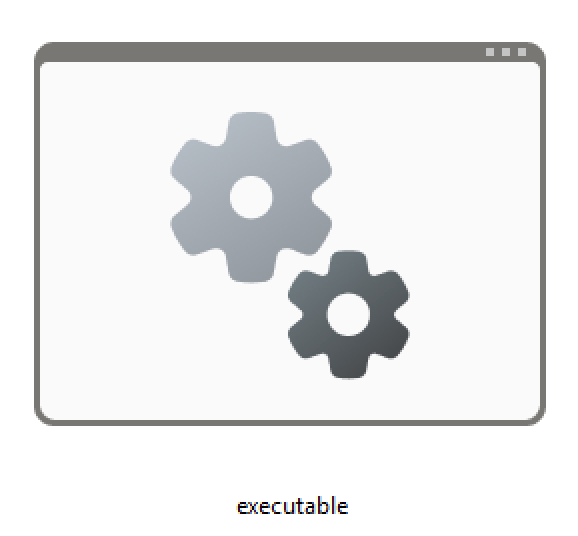
\includegraphics[width=0.4\textwidth]{figs/windows_executable.png}
	\caption{Running \texttt{executable.bat} from the project's root directory on Windows.}
	\label{fig:windows-executable}
\end{figure}

If any dependency is missing, the script will display instructions in the terminal. For example, it may indicate that Python or Graphviz must be installed, or that PowerShell should be run with administrator privileges. In that case, the user should follow the displayed instructions, close the window if necessary, and run \texttt{executable.bat} again.

\subsubsection{Running on macOS and Linux}

On macOS and Linux, users must open the project's root directory and execute:

\begin{verbatim}
	executable.command
\end{verbatim}

On macOS, this file can be opened by double-clicking it in Finder. On Linux, depending on the file manager and system configuration, it can be opened either by double-clicking or by selecting the option to run it as a program.

If the system indicates that the file does not have execution permissions, permission must be granted once. This can be done through the file properties in the file explorer by enabling execution permissions. It can also be done from a terminal using:

\begin{verbatim}
	chmod +x executable.command
\end{verbatim}

Once executed, the file internally calls:

\begin{verbatim}
	setup/setup_and_run.sh
\end{verbatim}

This script detects whether the operating system is macOS or Linux and performs the following actions:

\begin{enumerate}
	\item Locates the project root directory.
	\item Checks whether Python 3.10 or later is installed.
	\item Checks whether Tkinter is available.
	\item Checks whether Graphviz is installed and whether the \texttt{dot} command is available.
	\item Creates or reuses the \texttt{.venv} virtual environment.
	\item Installs the dependencies listed in \texttt{requirements.txt}.
	\item Executes \texttt{tools/check\_environment.py}.
	\item If everything is correct, launches \texttt{src/GUI.py}.
\end{enumerate}

\begin{figure}[H]
	\centering
	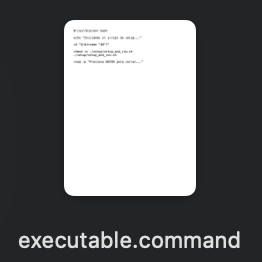
\includegraphics[width=0.4\textwidth]{figs/macos_executable.png}
	\caption{Running \texttt{executable.command} from Finder on macOS.}
	\label{fig:macos-executable}
\end{figure}

On Linux, an equivalent screenshot may show the \texttt{executable.command} file within the file manager or the terminal window that opens during execution.

\subsubsection{Permissions and System Dependencies}

Although the executables automate most of the process, some dependencies may require special operating system permissions. This depends on the system configuration.

On Windows, if Python or Graphviz is not installed, the script may display installation commands using \texttt{winget}. If those commands require administrator privileges, a message will instruct the user to open PowerShell as an administrator and execute the indicated commands.

On macOS, if Homebrew, Python, or Graphviz is missing, the script will display installation instructions. In some cases, Homebrew must be installed before proceeding.

On Linux, if system dependencies are missing, the script may suggest commands using \texttt{sudo}, for example to install Python, Tkinter, or Graphviz. If a password prompt appears, it refers to the password of a user with administrative privileges.

The purpose of these scripts is to avoid silent or confusing installations. Therefore, whenever elevated permissions are required, the process informs the user before continuing.

\subsection{Expected Output}

If everything is configured correctly, the terminal should display messages similar to the following:

\begin{verbatim}
	[INFO] Project detected at: .../PENTA-Compiler
	[INFO] Operating system detected: ...
	[OK] Python detected: Python 3.x.x
	[OK] Graphviz detected: dot - graphviz version ...
	[OK] Virtual environment .venv already exists.
	[INFO] Installing Python dependencies...
	[INFO] Running environment checker...
	[OK] Environment ready. Launching PENTA Compiler...
\end{verbatim}

After this output, the main PENTA Compiler window should open.

\begin{figure}[H]
	\centering
	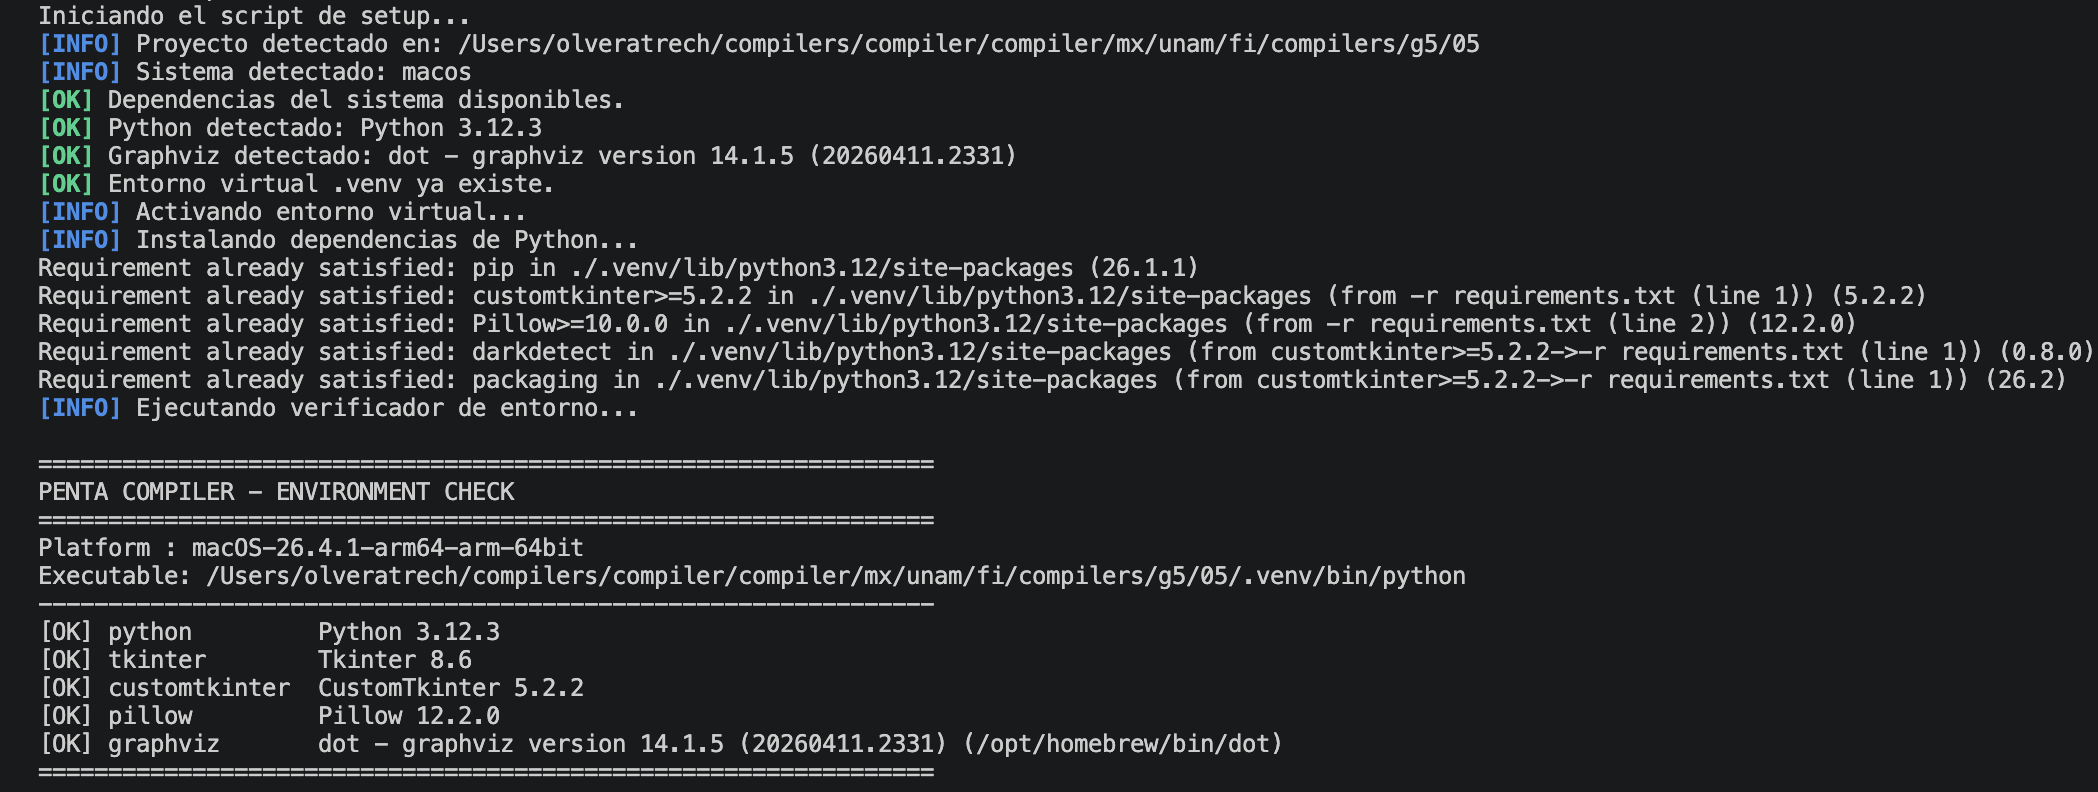
\includegraphics[width=\textwidth]{figs/successful_terminal_output.png}
	\caption{Expected terminal output when the environment is successfully validated.}
	\label{fig:successful-terminal-output}
\end{figure}

\begin{figure}[H]
	\centering
	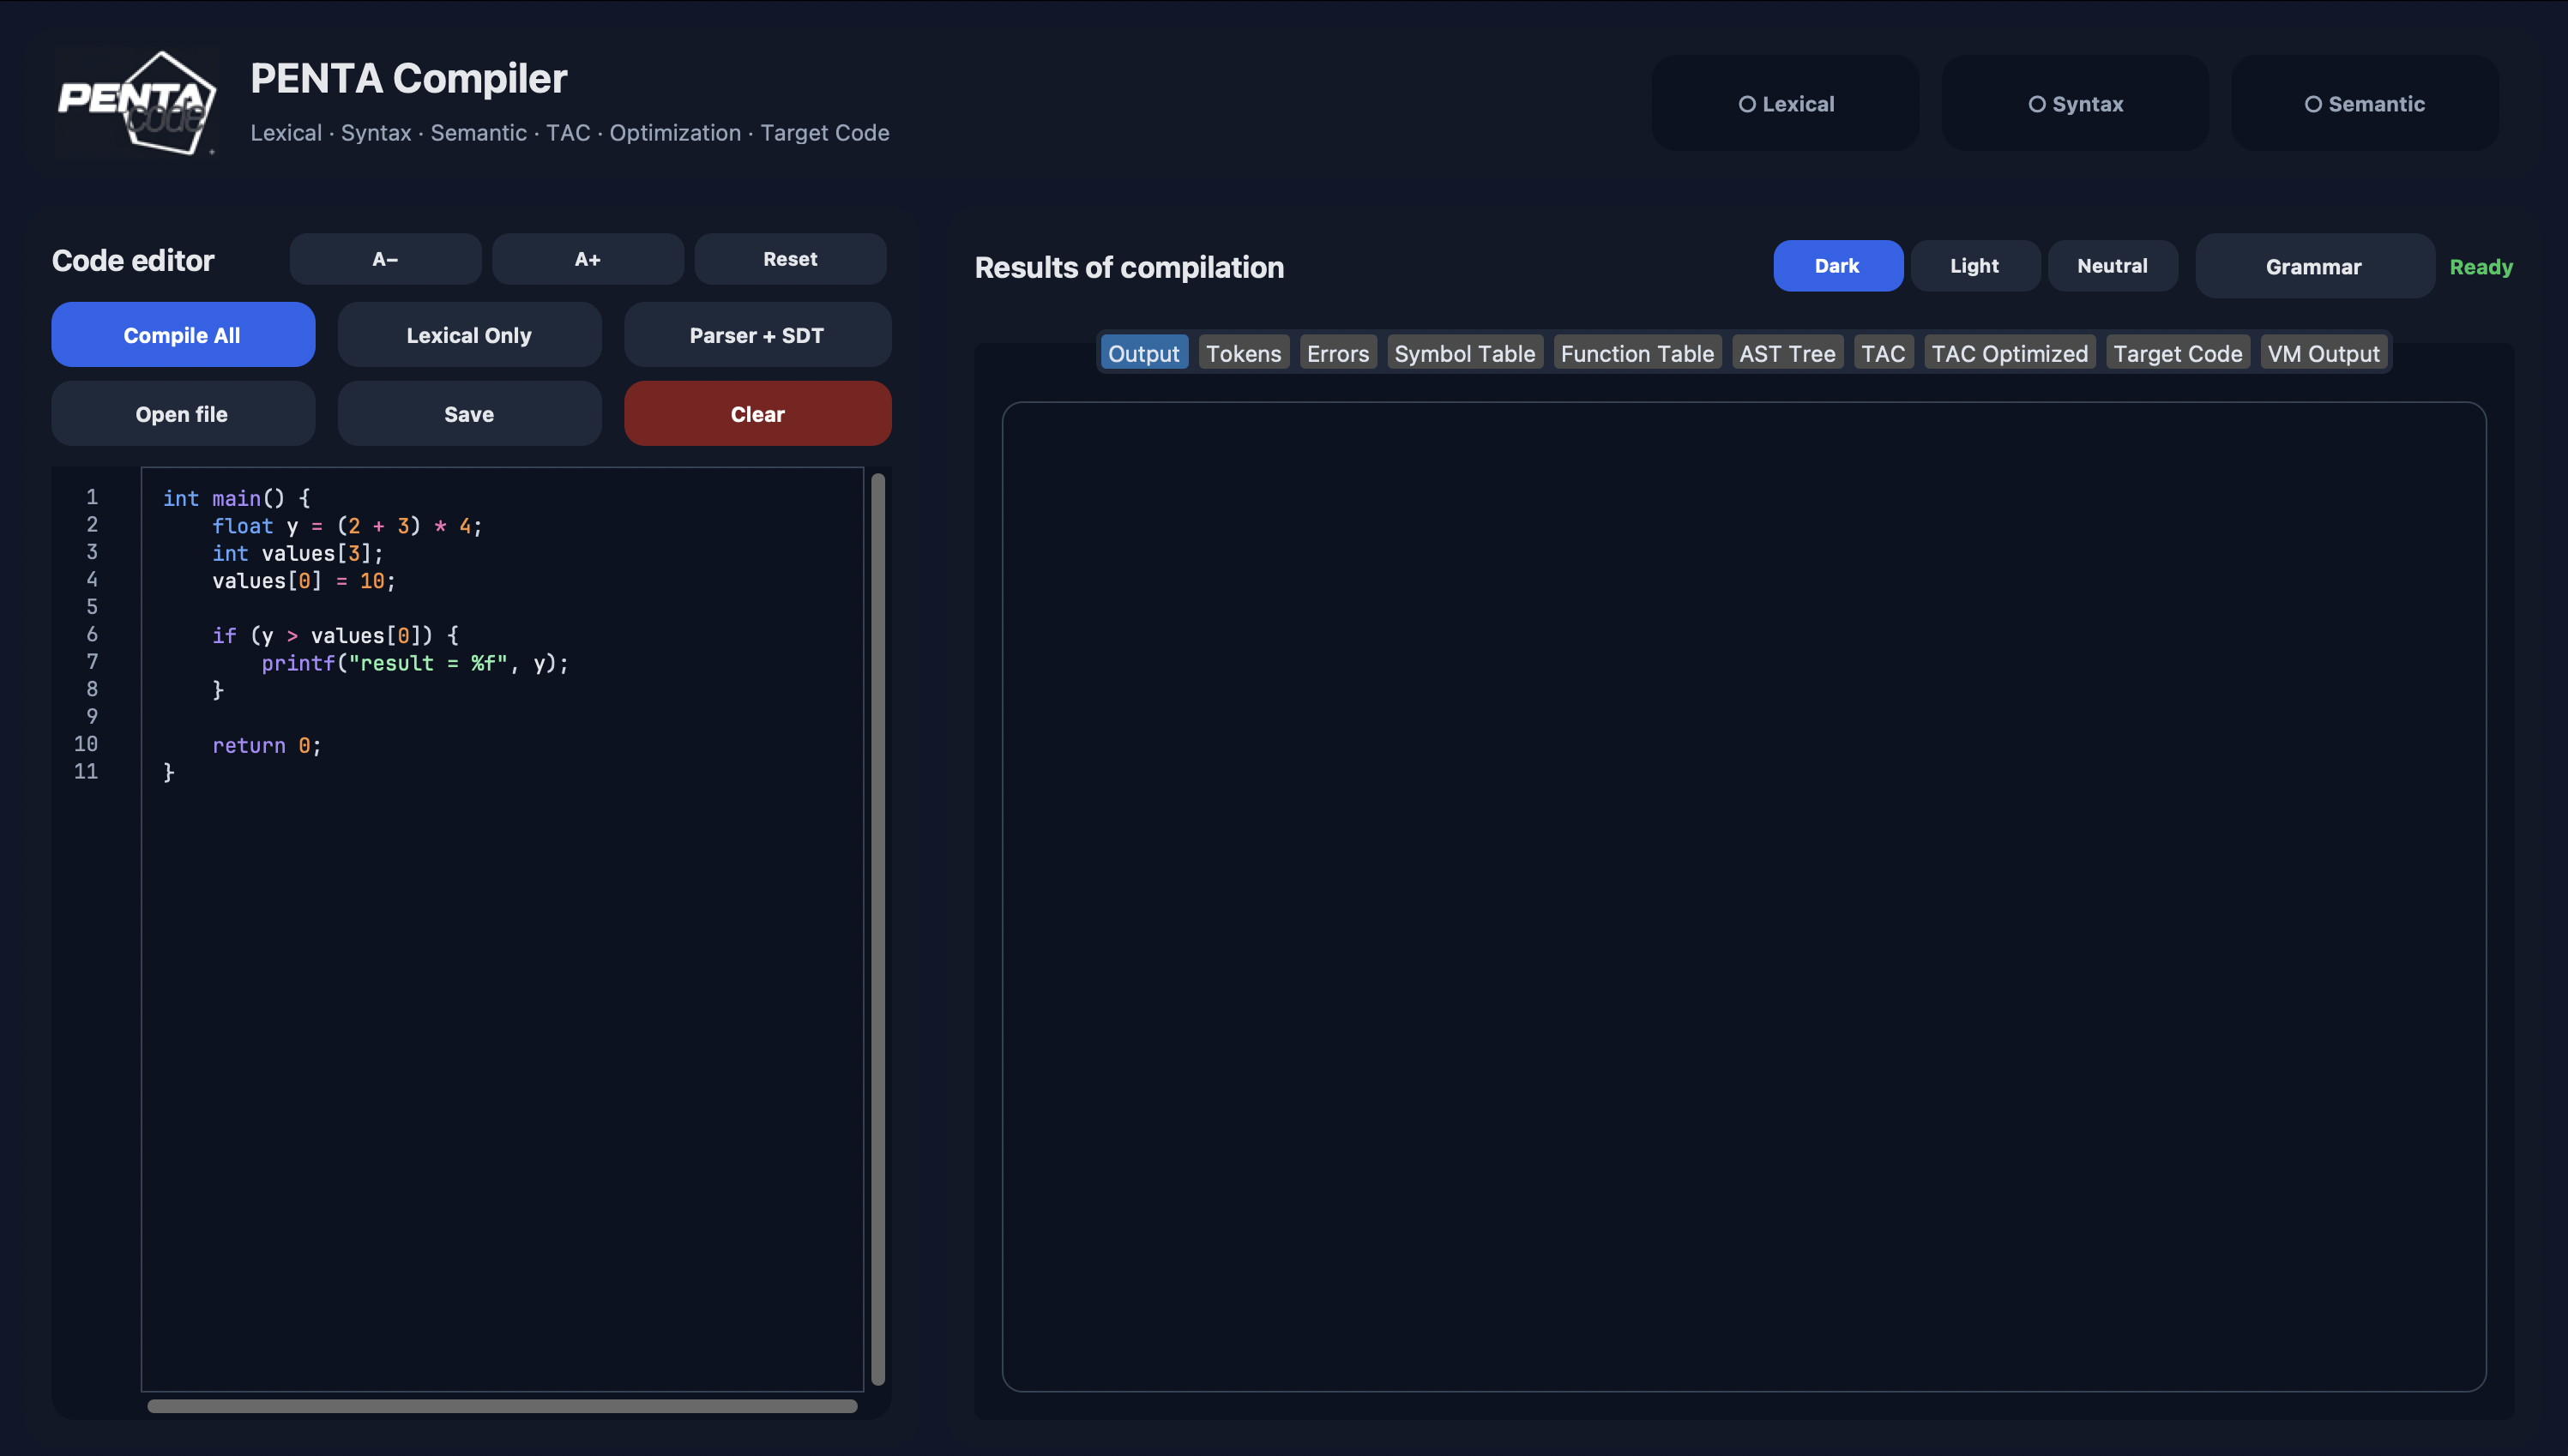
\includegraphics[width=\textwidth]{figs/gui_opened.png}
	\caption{PENTA Compiler graphical interface opened after running the automated executable.}
	\label{fig:gui-opened}
\end{figure}

\subsubsection{What to Do If an Error Occurs}

If the process stops, the message displayed in the terminal should be read carefully. The most common cases are:

\begin{itemize}
	\item \textbf{The file does not execute}: verify that it is being run from the project root directory and that the \texttt{setup/} directory exists.
	\item \textbf{Python is missing}: install Python 3.10 or later and run the file again.
	\item \textbf{Graphviz is missing}: install Graphviz and verify that the \texttt{dot} command is available.
	\item \textbf{Tkinter is missing}: install the package corresponding to the operating system.
	\item \textbf{Insufficient permissions}: follow the instructions displayed by the script in the terminal.
	\item \textbf{PowerShell blocks scripts}: run \texttt{executable.bat} again, as it applies a temporary execution policy to avoid this restriction.
	\item \textbf{\texttt{executable.command} does not open}: grant execution permissions to the file and try again.
\end{itemize}

After correcting the indicated issue, the corresponding executable should be run again.

\subsubsection{Execution Summary}

The execution workflow for the end user is simplified as follows:

\begin{itemize}
	\item On Windows: double-click \texttt{executable.bat}.
	\item On macOS or Linux: execute \texttt{executable.command}.
\end{itemize}

\subsection{Valid Test Cases}
\subsubsection{Test Case 1: Valid Declaration, Arrays, Arithmetic Operations and Control Structures}
Figure 1 shows the source code input, which consists of variable declarations, arrays, arithmetic operations, and control structures. It also displays the available options for processing the code with our program (compile, lexical analyzer, syntactic analyzer, load files, and save).\\
Figure 2 shows the validation of its execution through all the compiler phases, as well as the output generated in the VM. The other images (Figure 3, 4, 5, 6, 7, 8, 9, 10, 11) show the output after passing through each compiler phase.
\begin{figure}[H]
	\centering
	\begin{minipage}[t]{0.48\textwidth}
		\centering
		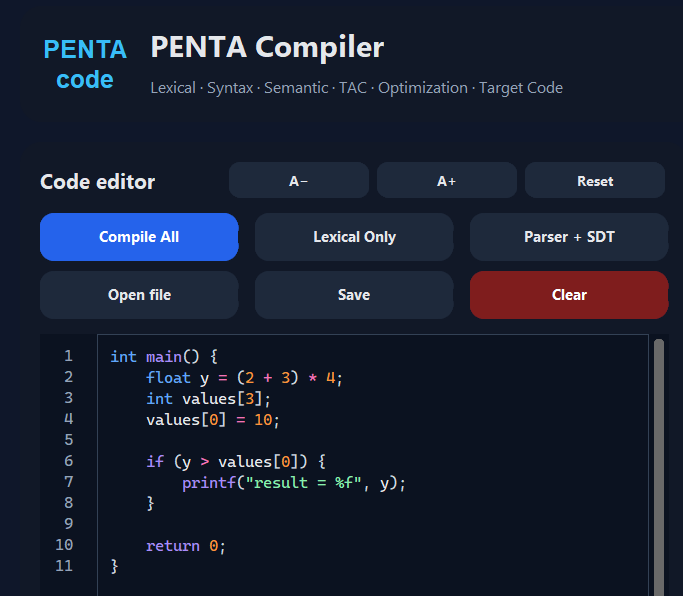
\includegraphics[width=\textwidth]{figs/test1_input.png}
		\caption{Input for Test Case 1}
		\label{fig:test1}
	\end{minipage}
	\hfill
	\begin{minipage}[t]{0.48\textwidth}
		\centering
		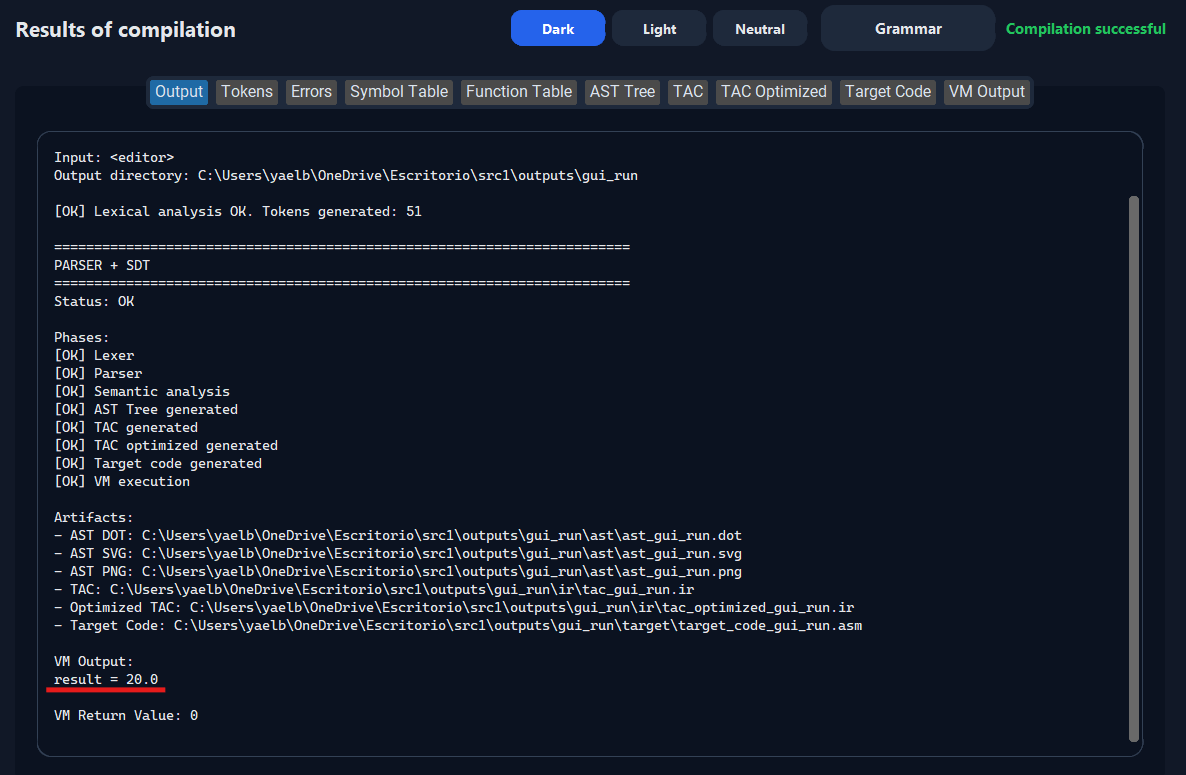
\includegraphics[width=\textwidth]{figs/test1_output.png}
		\caption{Output for Test Case 1}
		\label{fig:test1_ast}
	\end{minipage}
\end{figure}

\begin{figure}[H]
	\centering
	\begin{minipage}[t]{0.32\textwidth}
		\centering
		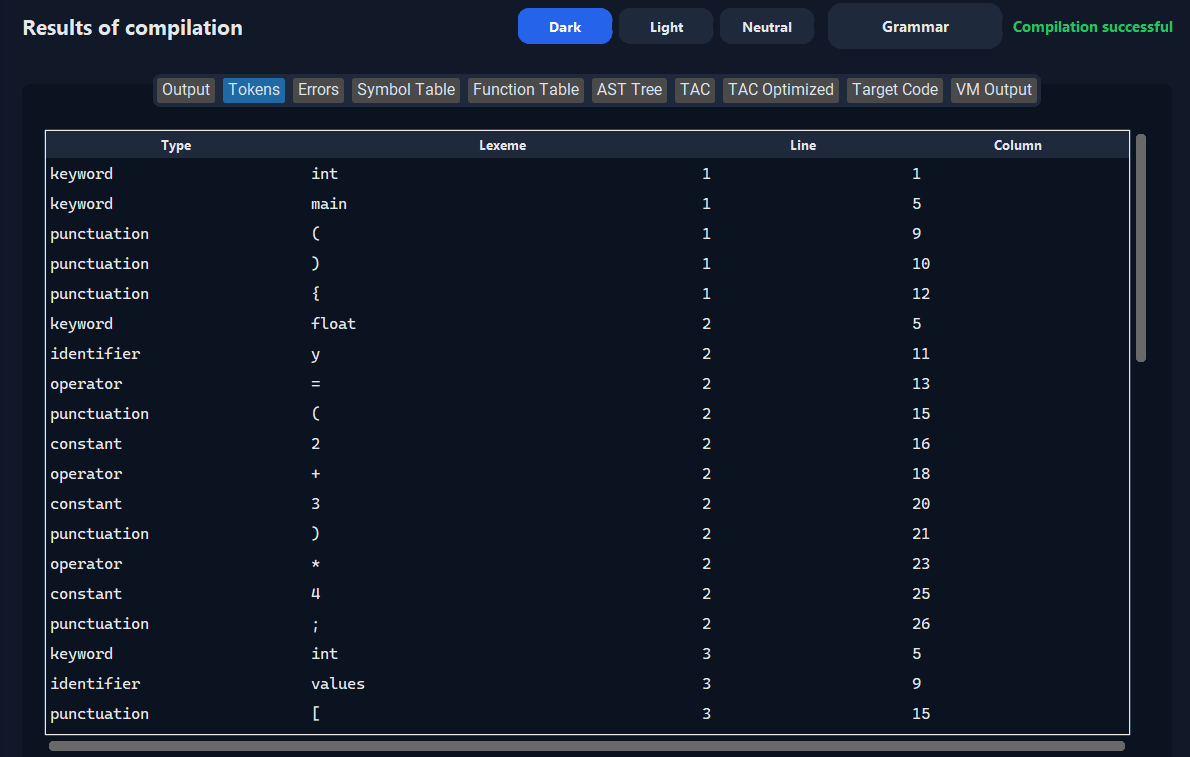
\includegraphics[width=\textwidth]{figs/test1_output1.png}
		\caption{Tokens}
		\label{fig:test1}
	\end{minipage}
	\hfill
	\begin{minipage}[t]{0.32\textwidth}
		\centering
		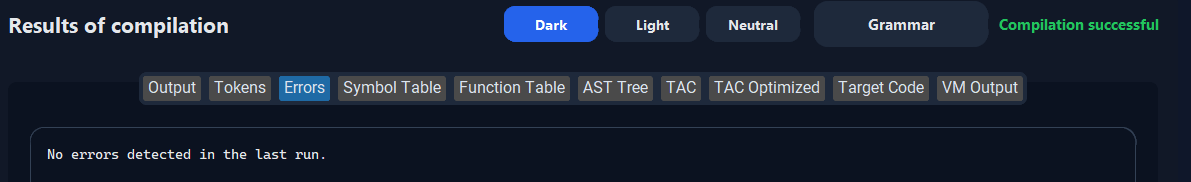
\includegraphics[width=\textwidth]{figs/test1_output2.png}
		\caption{Errors}
		\label{fig:test1_ast}
	\end{minipage}
    \hfill
	\begin{minipage}[t]{0.32\textwidth}
		\centering
		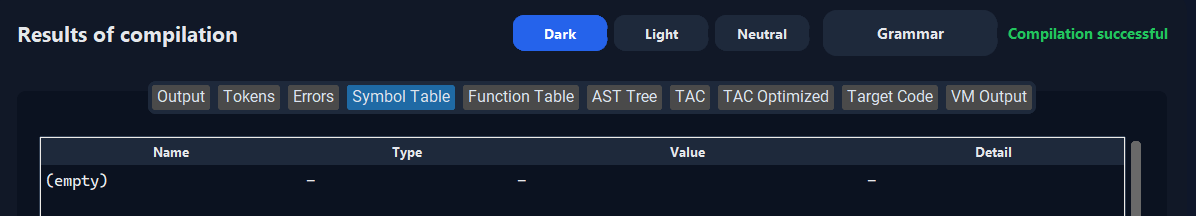
\includegraphics[width=\textwidth]{figs/test1_output3.png}
		\caption{Symbol Table}
		\label{fig:test1_ast}
	\end{minipage}

    \vspace{0.4cm}

    \begin{minipage}[t]{0.32\textwidth}
		\centering
		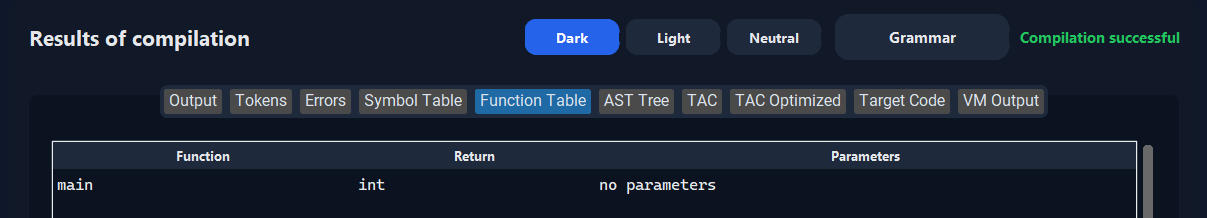
\includegraphics[width=\textwidth]{figs/test1_output4.png}
		\caption{Function Table}
		\label{fig:test1}
	\end{minipage}
	\hfill
	\begin{minipage}[t]{0.32\textwidth}
		\centering
		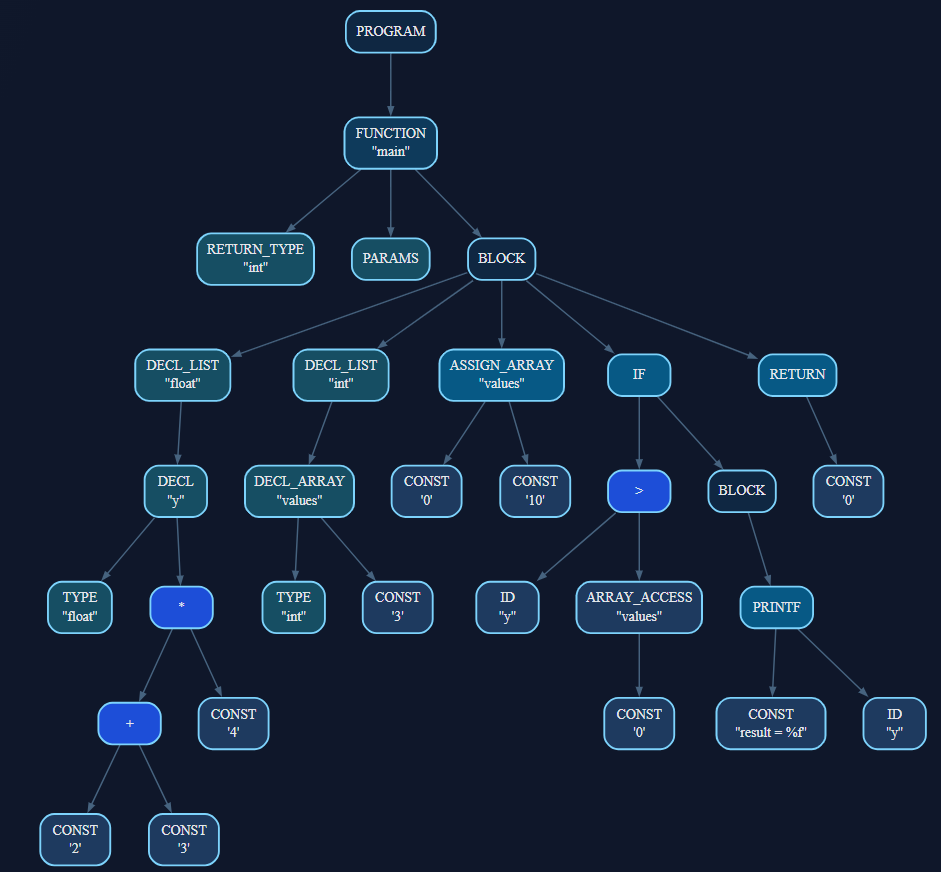
\includegraphics[width=\textwidth]{figs/test1_outputAST.png}
		\caption{AST Tree}
		\label{fig:test1_ast}
	\end{minipage}
    \hfill
	\begin{minipage}[t]{0.32\textwidth}
		\centering
		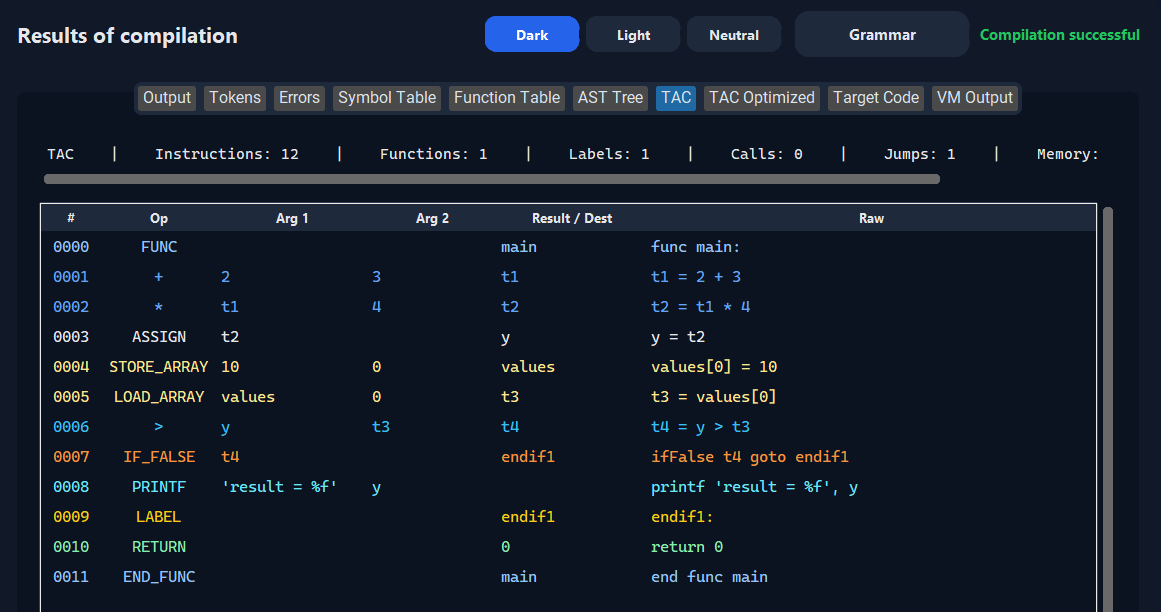
\includegraphics[width=\textwidth]{figs/test1_outputTAC.png}
		\caption{TAC}
		\label{fig:test1_ast}
	\end{minipage}

    \vspace{0.4cm}

    \begin{minipage}[t]{0.32\textwidth}
		\centering
		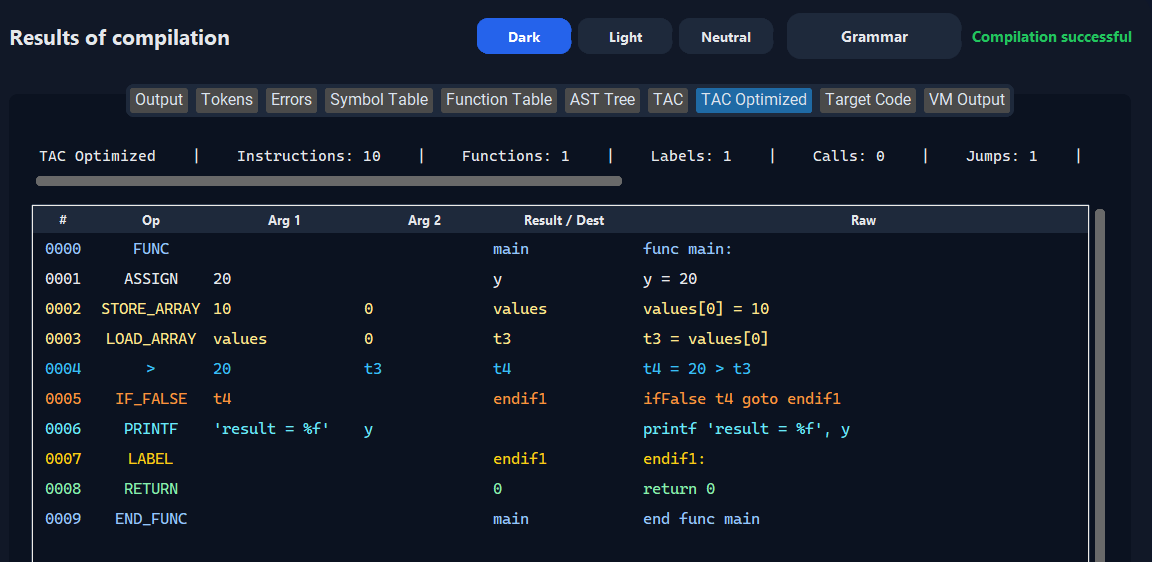
\includegraphics[width=\textwidth]{figs/test1_outputTACO.png}
		\caption{TAC Optimized}
		\label{fig:test1}
	\end{minipage}
	\hfill
	\begin{minipage}[t]{0.32\textwidth}
		\centering
		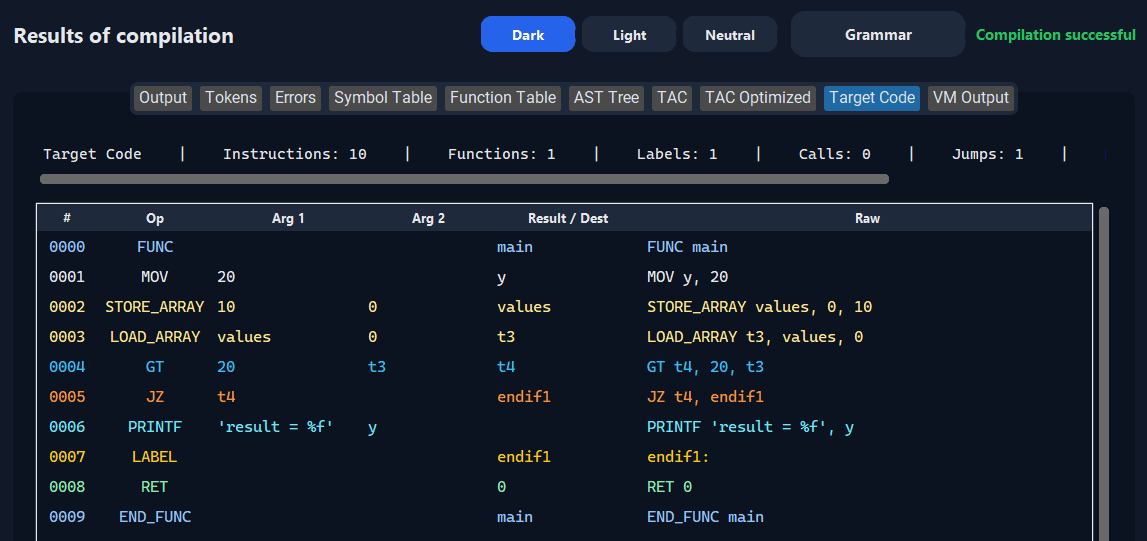
\includegraphics[width=\textwidth]{figs/test1_outputTarg.png}
		\caption{Target Code}
		\label{fig:test1_ast}
	\end{minipage}
    \hfill
	\begin{minipage}[t]{0.32\textwidth}
		\centering
		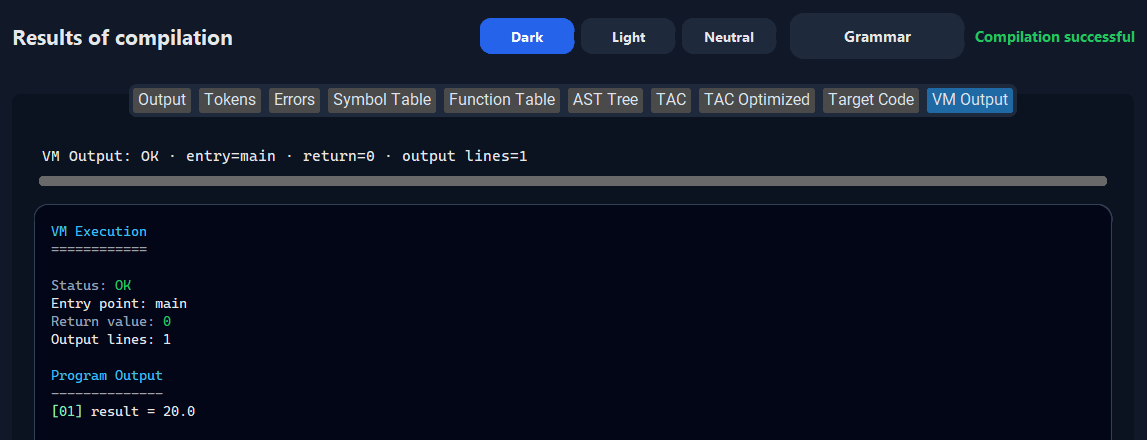
\includegraphics[width=\textwidth]{figs/test1_outputVM.png}
		\caption{VM Output}
		\label{fig:test1_ast}
	\end{minipage}
\end{figure}

\subsubsection{Test Case 2: Valid Declarations, Arrays, Indexes, and Functions (05\_function\_param\_index\_ok.c)}
Figure 12 shows the input source code, which consists of variable declarations, arrays, indices, functions, and parameters. It also shows the available options for processing the code with our program (compile, lexical analyzer, parser, load files, and save). Figure 13 shows the validation of its execution through all the compiler phases, as well as the output generated in the virtual machine. The remaining figures (14, 15, 16, 17, 18, 19, 20, 21, and 22) show the output after passing through each compiler phase.

\begin{figure}[H]
	\centering
	\begin{minipage}[t]{0.48\textwidth}
		\centering
		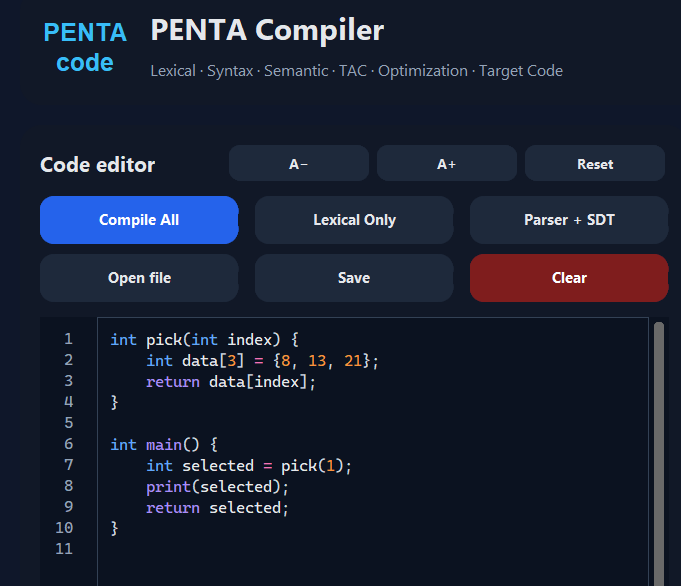
\includegraphics[width=\textwidth]{figs/test2_input.png}
		\caption{Input for Test Case 2}
		\label{fig:test1}
	\end{minipage}
	\hfill
	\begin{minipage}[t]{0.48\textwidth}
		\centering
		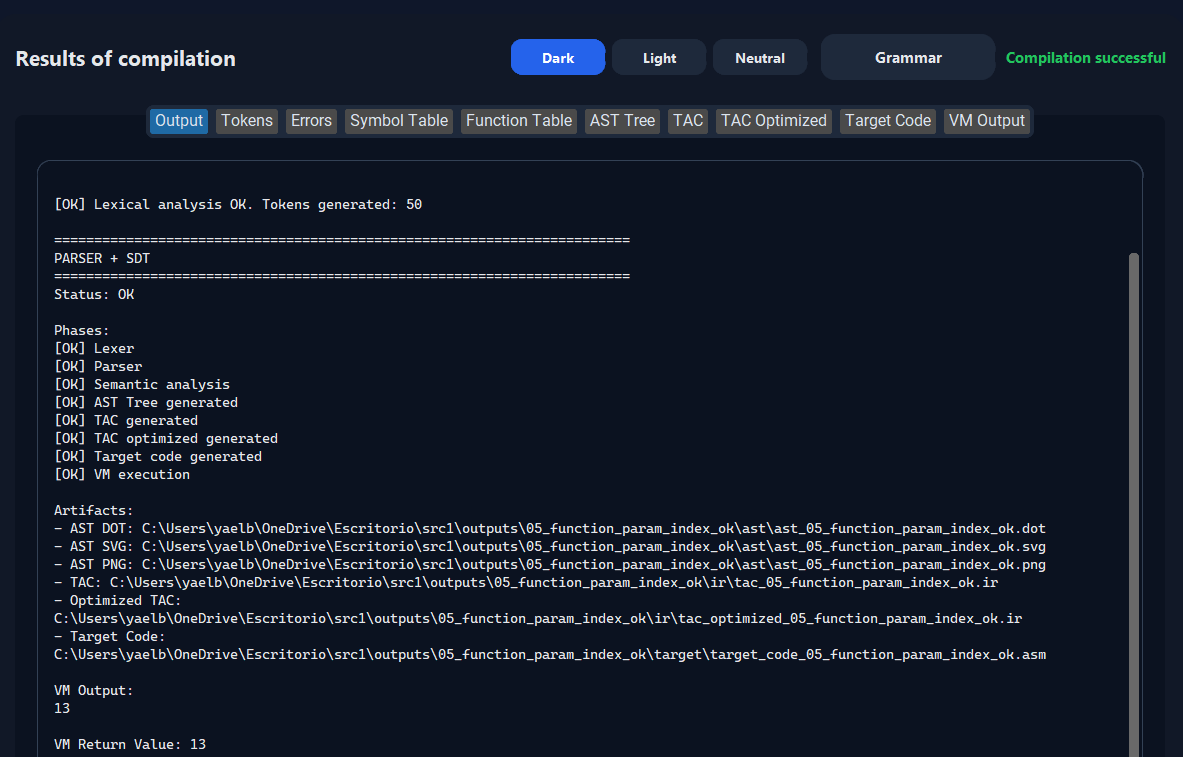
\includegraphics[width=\textwidth]{figs/test2_output.png}
		\caption{Output for Test Case 2}
		\label{fig:test1_ast}
	\end{minipage}

    \vspace{0.4cm}

    \begin{minipage}[t]{0.32\textwidth}
		\centering
		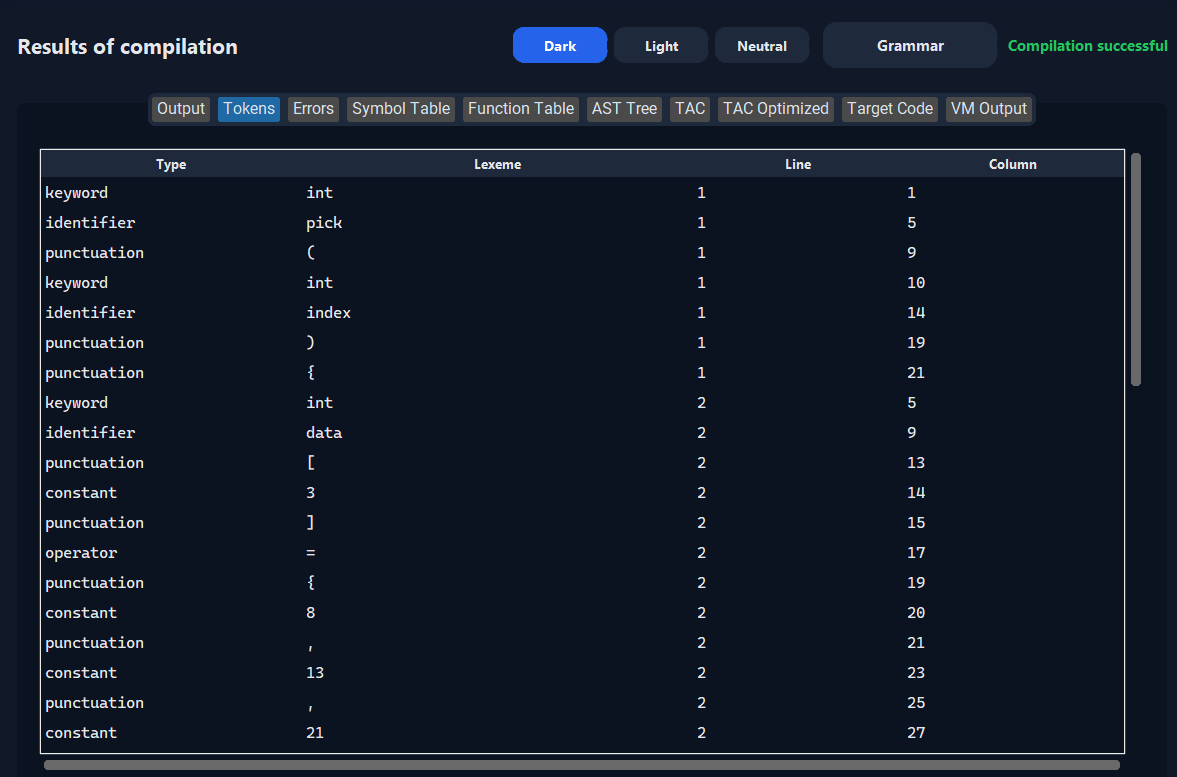
\includegraphics[width=\textwidth]{figs/test2_output1.png}
		\caption{Tokens}
		\label{fig:test1}
	\end{minipage}
	\hfill
	\begin{minipage}[t]{0.32\textwidth}
		\centering
		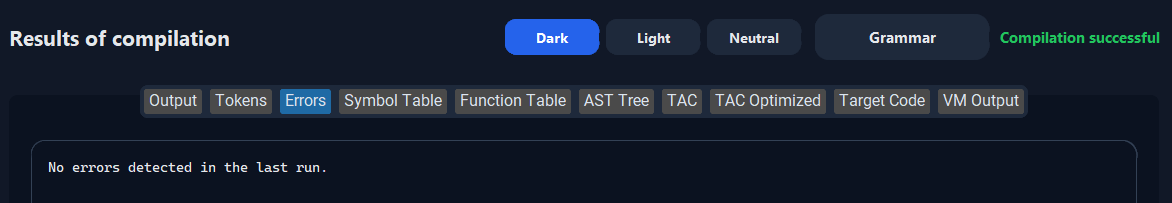
\includegraphics[width=\textwidth]{figs/test2_output2.png}
		\caption{Errors}
		\label{fig:test1_ast}
	\end{minipage}
    \hfill
	\begin{minipage}[t]{0.32\textwidth}
		\centering
		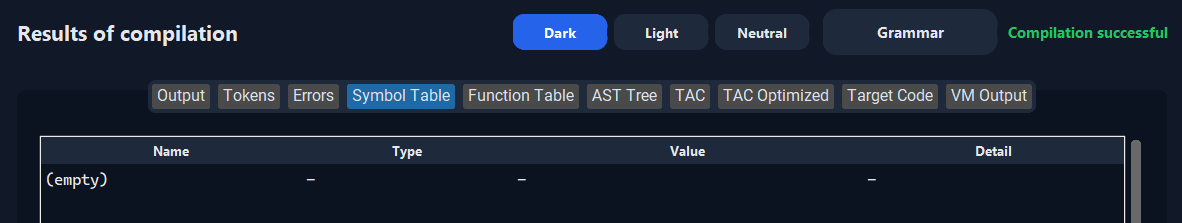
\includegraphics[width=\textwidth]{figs/test2_output3.png}
		\caption{Symbol Table}
		\label{fig:test1_ast}
	\end{minipage}

    \vspace{0.4cm}

    \begin{minipage}[t]{0.32\textwidth}
		\centering
		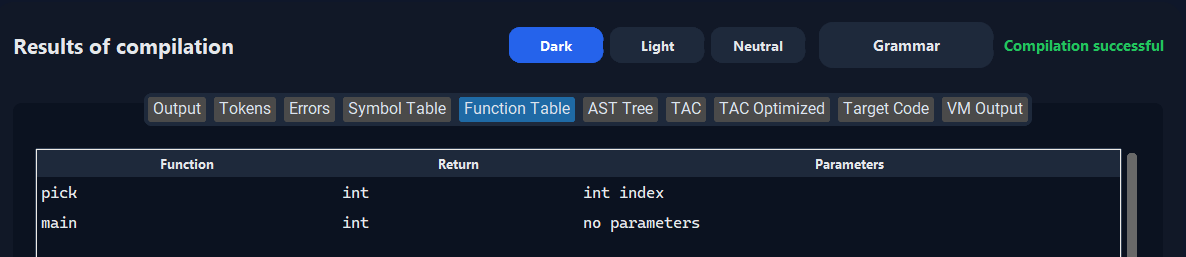
\includegraphics[width=\textwidth]{figs/test2_output4.png}
		\caption{Function Table}
		\label{fig:test1}
	\end{minipage}
	\hfill
	\begin{minipage}[t]{0.32\textwidth}
		\centering
		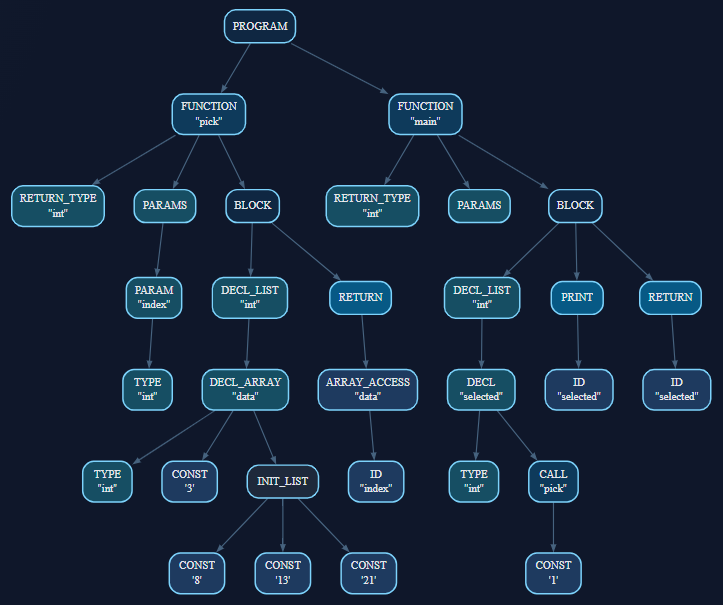
\includegraphics[width=\textwidth]{figs/test2_outputAST.png}
		\caption{AST Tree}
		\label{fig:test1_ast}
	\end{minipage}
    \hfill
	\begin{minipage}[t]{0.32\textwidth}
		\centering
		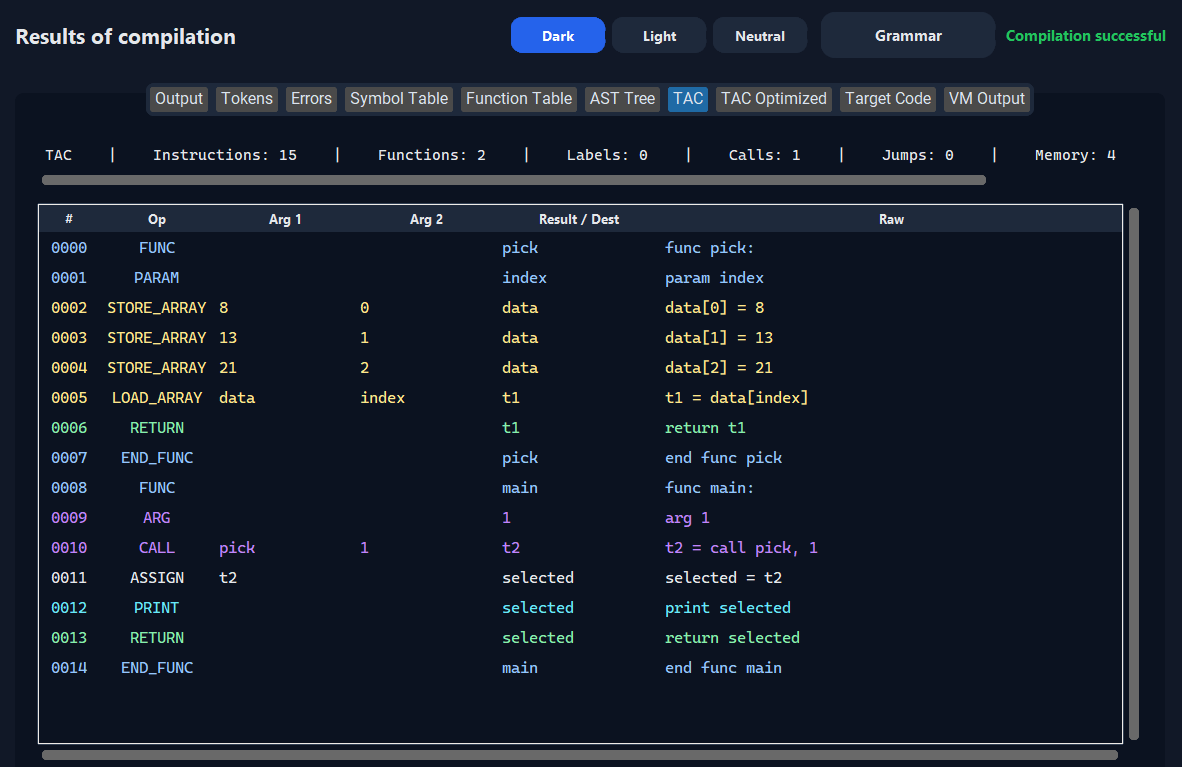
\includegraphics[width=\textwidth]{figs/test2_outputTAC.png}
		\caption{TAC}
		\label{fig:test1_ast}
	\end{minipage}
\end{figure}

\begin{figure}[H]
    \begin{minipage}[t]{0.32\textwidth}
		\centering
		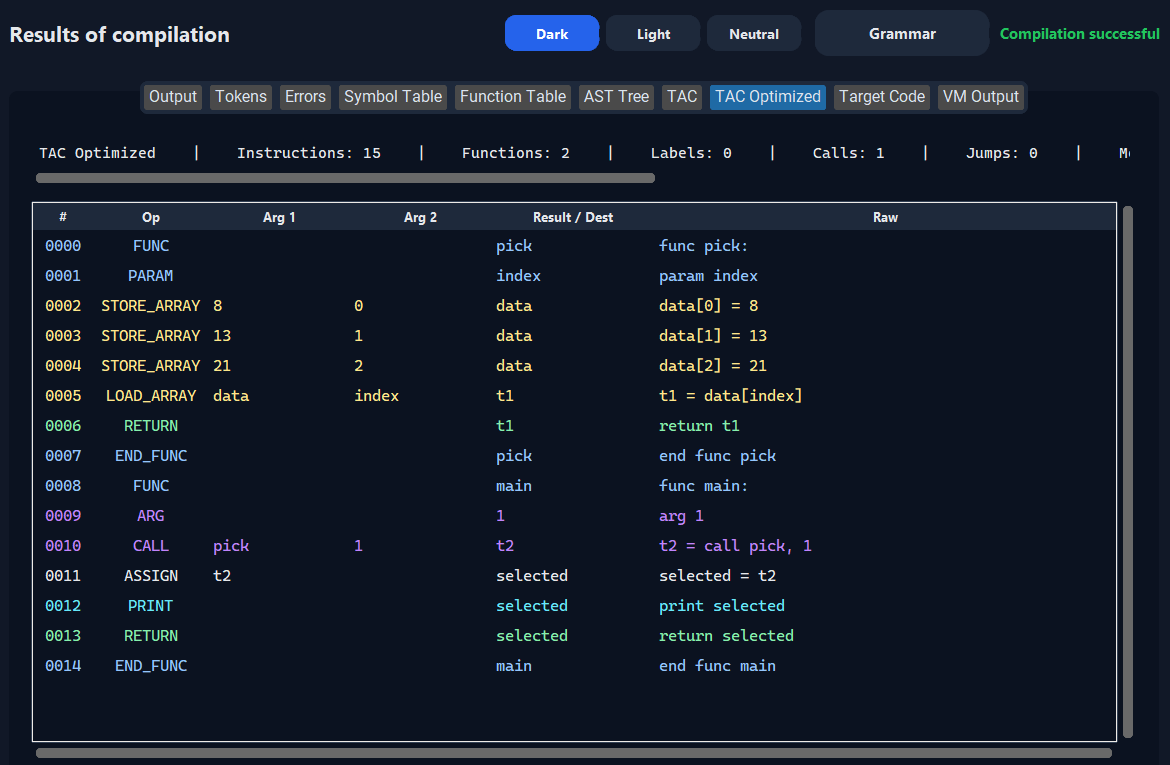
\includegraphics[width=\textwidth]{figs/test2_outputTACO.png}
		\caption{TAC Optimized}
		\label{fig:test1}
	\end{minipage}
	\hfill
	\begin{minipage}[t]{0.32\textwidth}
		\centering
		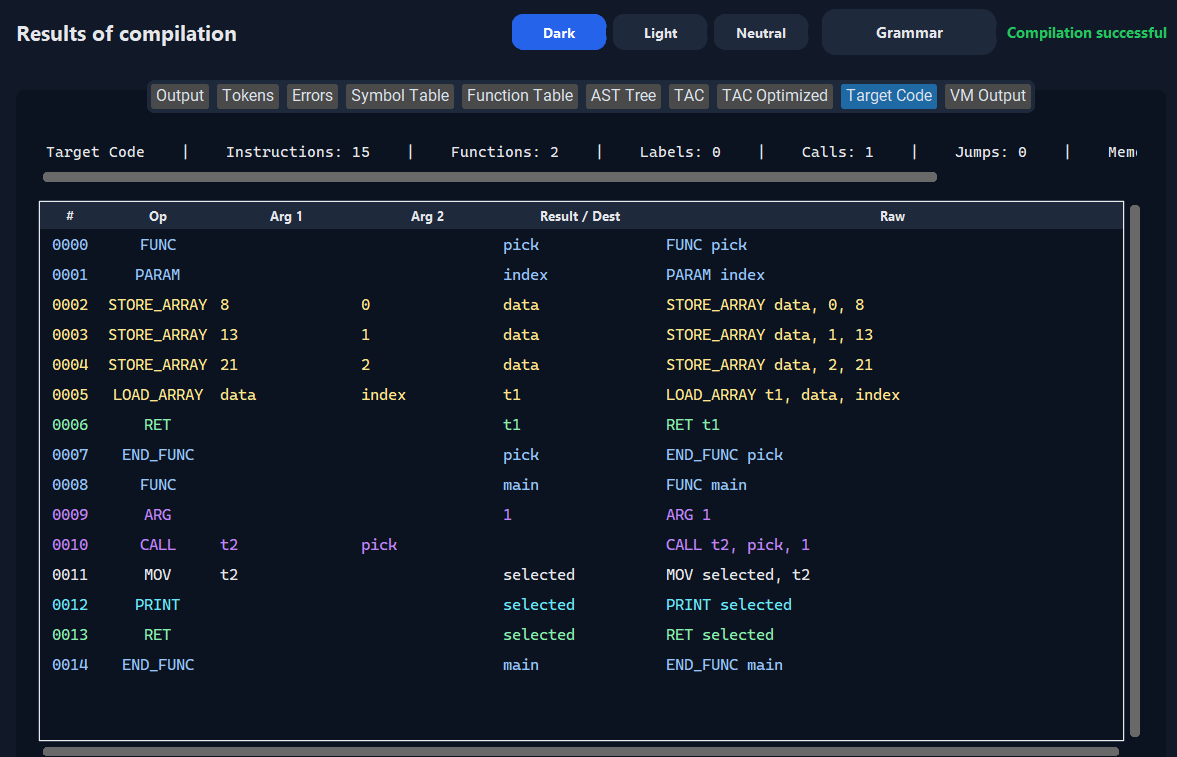
\includegraphics[width=\textwidth]{figs/test2_outputTarg.png}
		\caption{Target Code}
		\label{fig:test1_ast}
	\end{minipage}
    \hfill
	\begin{minipage}[t]{0.32\textwidth}
		\centering
		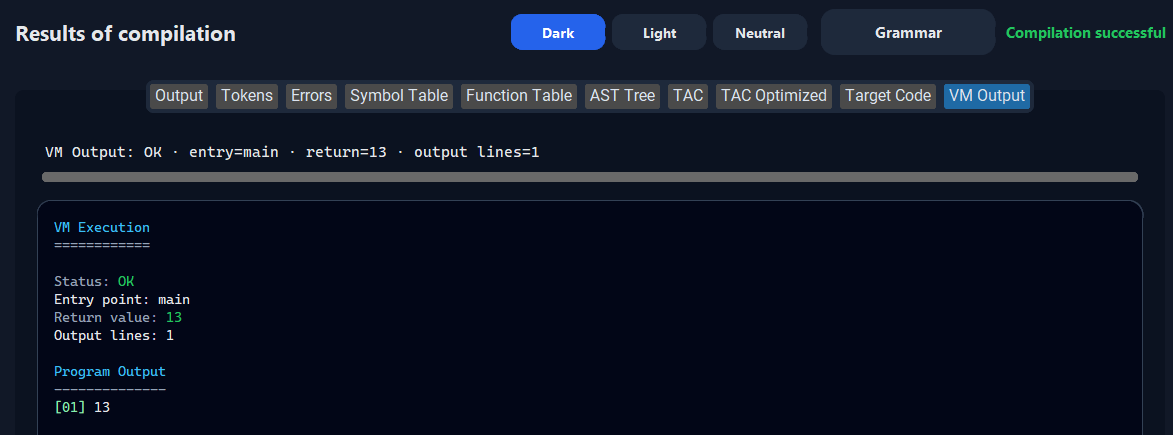
\includegraphics[width=\textwidth]{figs/test2_outputVM.png}
		\caption{VM Output}
		\label{fig:test1_ast}
	\end{minipage}
\end{figure}


\subsubsection{Test Case 3: Full Language Feature Integration  (05\_full\_feature\_succes.c)}
Figure 23 shows the input source code utilized for validating the compiler implementation. The test program integrates multiple language features, including variable declarations, arrays, function calls, arithmetic and logical operations, conditional and iterative control structures, semantic validations, and formatted output instructions. The figure also illustrates the main functionalities available in the compiler interface, such as compilation, lexical analysis, parsing, file loading, and file saving. Figure 24 shows the validation of its execution through all the compiler phases, as well as the output generated in the virtual machine. The remaining figures (25, 26, 27, 28, 29, 30, 31, 32, and 33) show the output after passing through each compiler phase.

\begin{figure}[H]
	\centering
	\begin{minipage}[t]{0.48\textwidth}
		\centering
		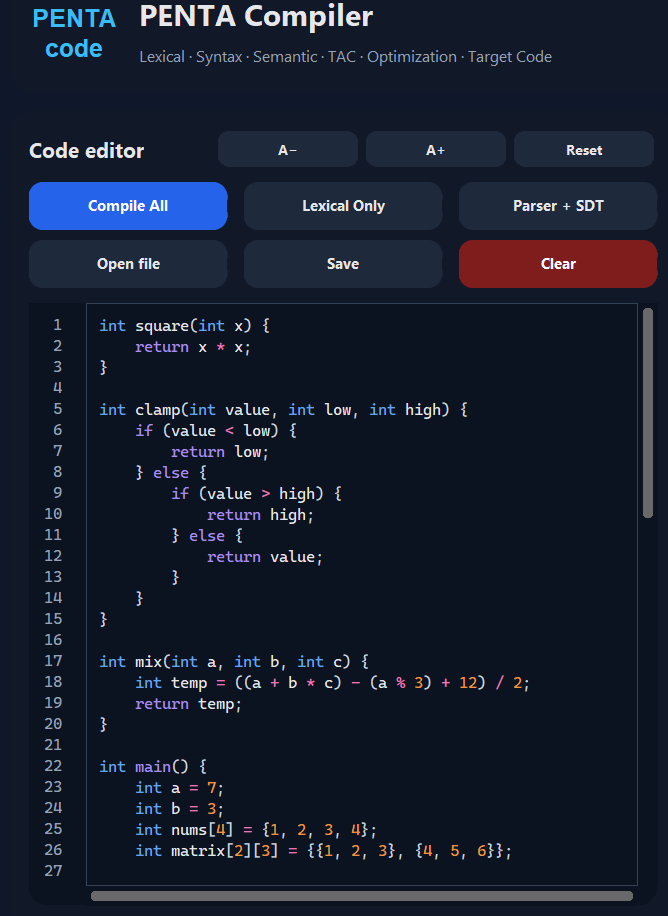
\includegraphics[width=\textwidth]{figs/test3_input.png}
		\caption{Input for Test Case 3}
		\label{fig:test1}
	\end{minipage}
	\hfill
	\begin{minipage}[t]{0.48\textwidth}
		\centering
		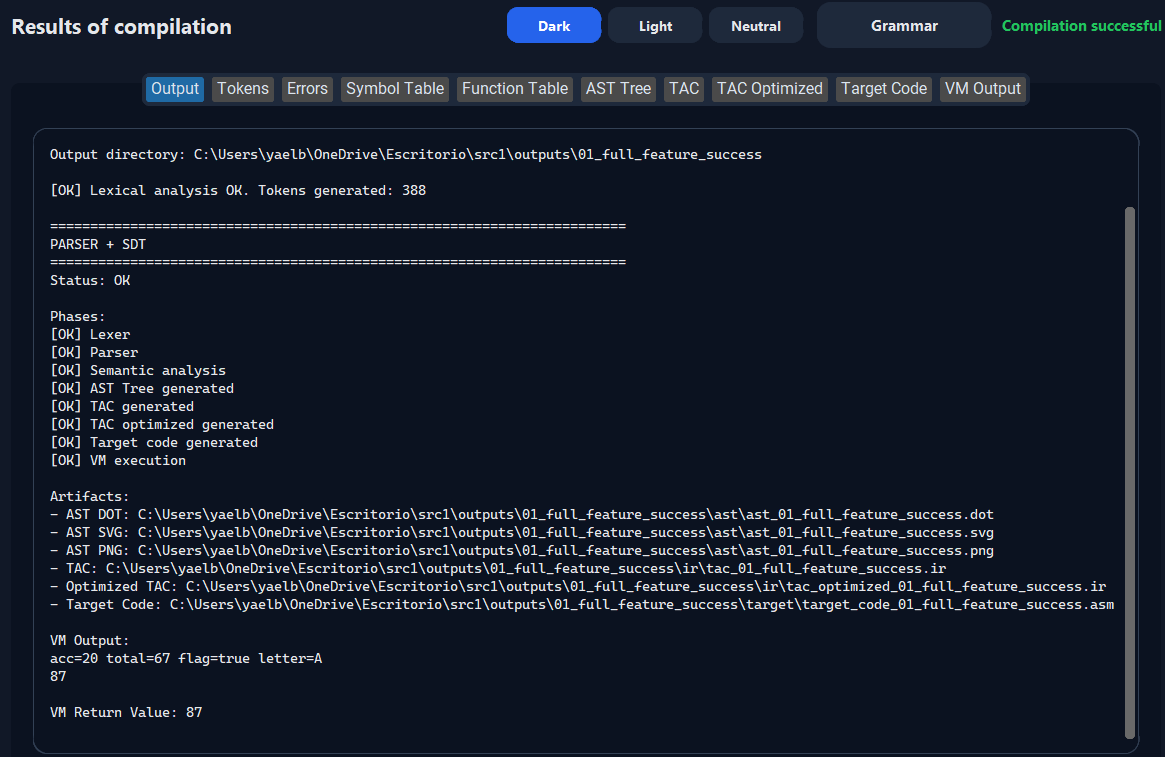
\includegraphics[width=\textwidth]{figs/test3_output.png}
		\caption{Output for Test Case 3}
		\label{fig:test1_ast}
	\end{minipage}
\end{figure}

\begin{figure}[H]
    \begin{minipage}[t]{0.32\textwidth}
		\centering
		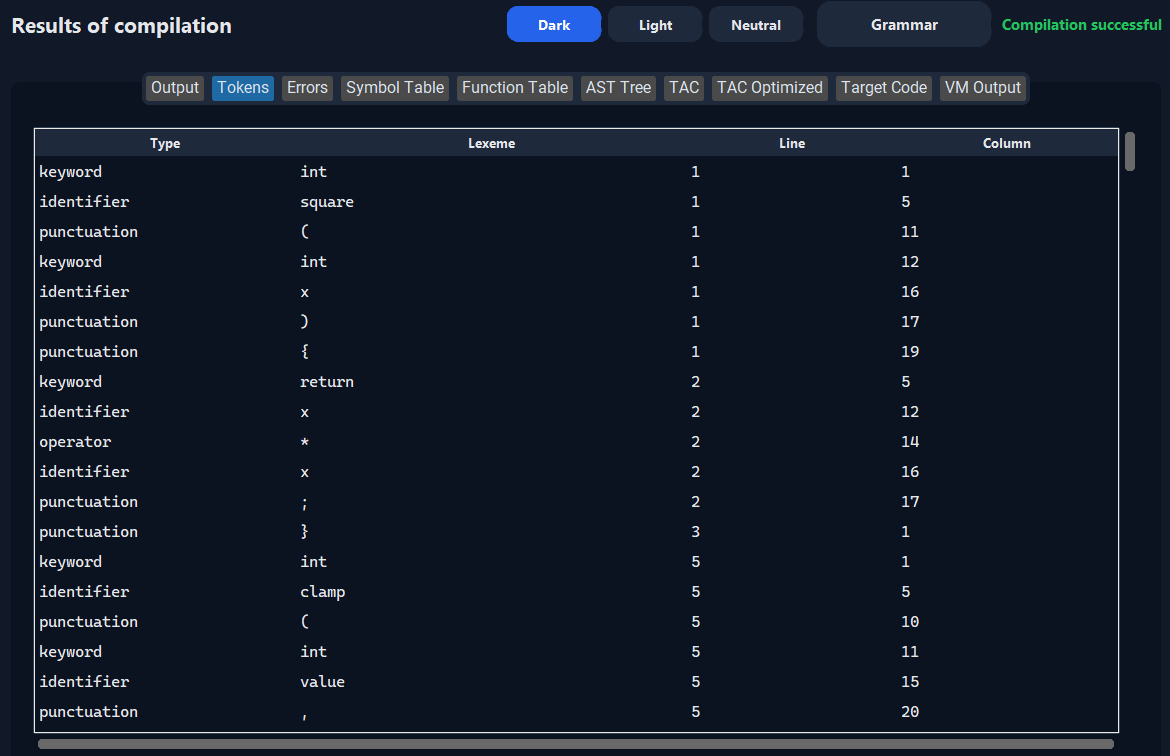
\includegraphics[width=\textwidth]{figs/test3_output1.png}
		\caption{Tokens}
		\label{fig:test1}
	\end{minipage}
	\hfill
	\begin{minipage}[t]{0.32\textwidth}
		\centering
		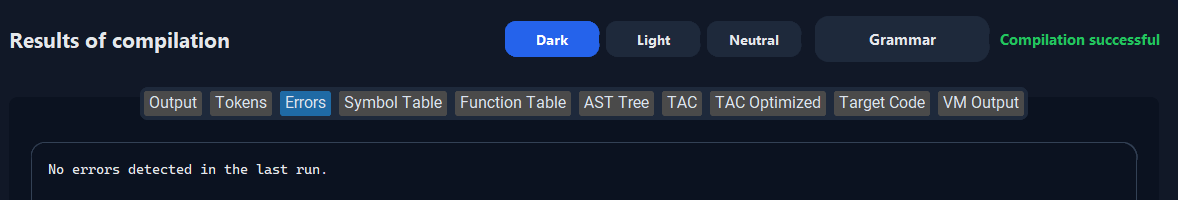
\includegraphics[width=\textwidth]{figs/test3_output2.png}
		\caption{Errors}
		\label{fig:test1_ast}
	\end{minipage}
    \hfill
	\begin{minipage}[t]{0.32\textwidth}
		\centering
		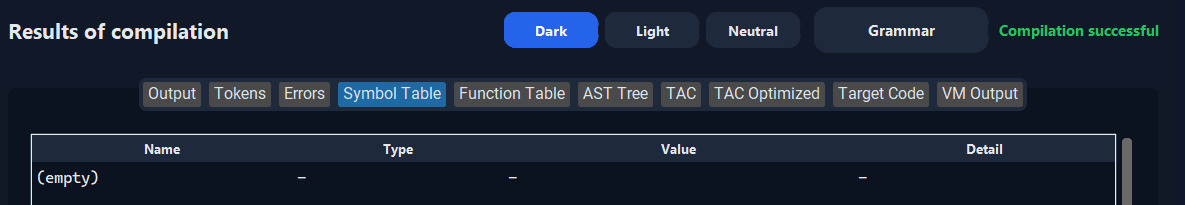
\includegraphics[width=\textwidth]{figs/test3_output3.png}
		\caption{Symbol Table}
		\label{fig:test1_ast}
	\end{minipage}

    \vspace{0.4cm}

    \begin{minipage}[t]{0.32\textwidth}
		\centering
		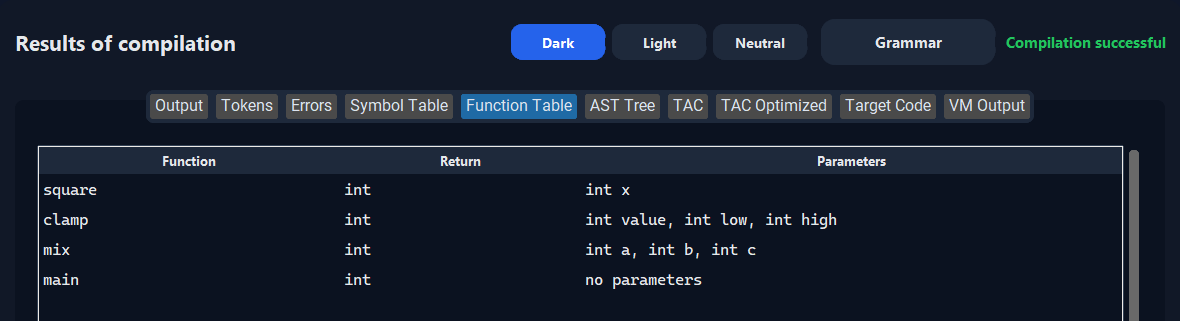
\includegraphics[width=\textwidth]{figs/test3_output4.png}
		\caption{Function Table}
		\label{fig:test1}
	\end{minipage}
	\hfill
	\begin{minipage}[t]{0.32\textwidth}
		\centering
		
\includegraphics[width=\textwidth]{figs/test3_outputAST.png}
		\caption{AST Tree}
		\label{fig:test1_ast}
	\end{minipage}
    \hfill
	\begin{minipage}[t]{0.32\textwidth}
		\centering
		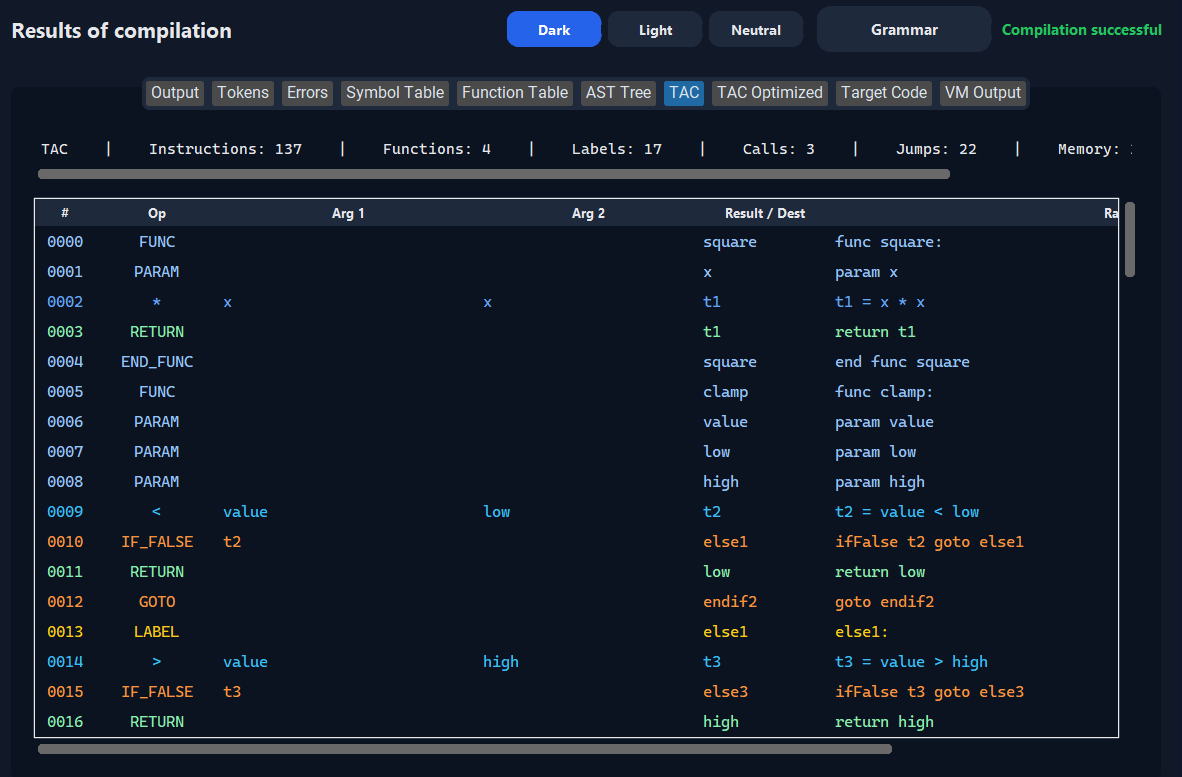
\includegraphics[width=\textwidth]{figs/test3_outputTAC.png}
		\caption{TAC}
		\label{fig:test1_ast}
	\end{minipage}

    \vspace{0.4cm}
    
    \begin{minipage}[t]{0.32\textwidth}
		\centering
		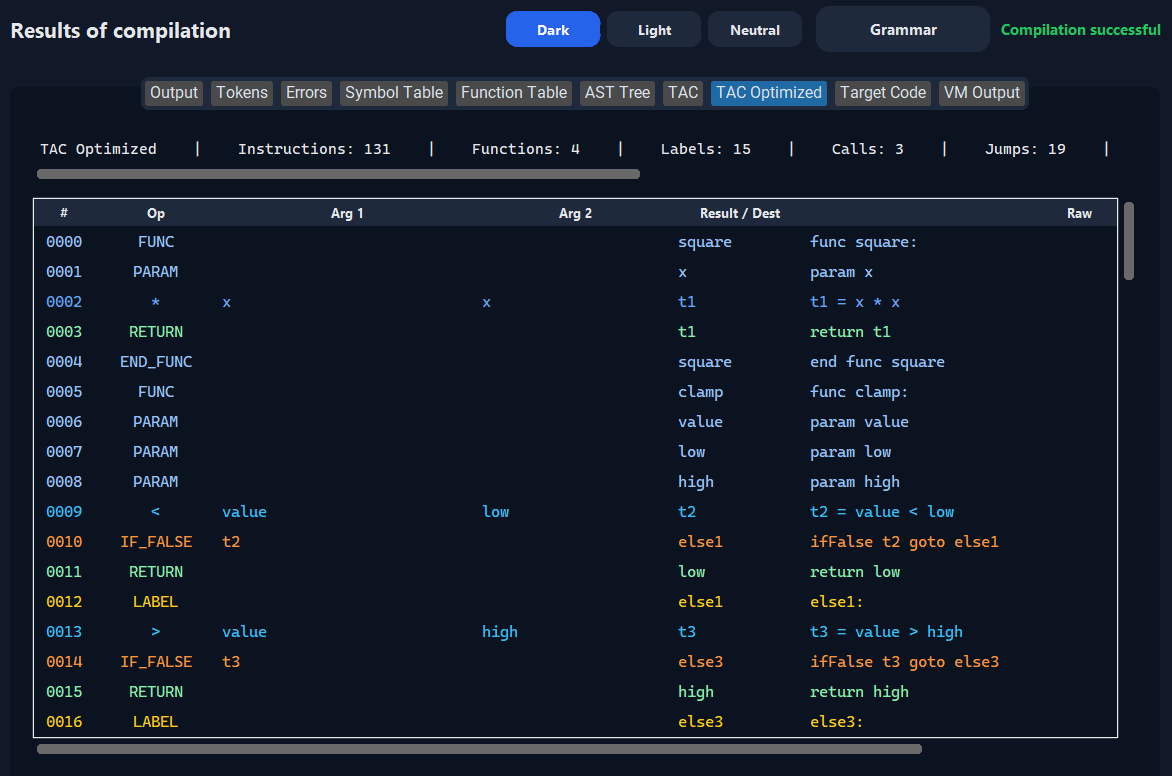
\includegraphics[width=\textwidth]{figs/test3_outputTACO.png}
		\caption{TAC Optimized}
		\label{fig:test1}
	\end{minipage}
	\hfill
	\begin{minipage}[t]{0.32\textwidth}
		\centering
		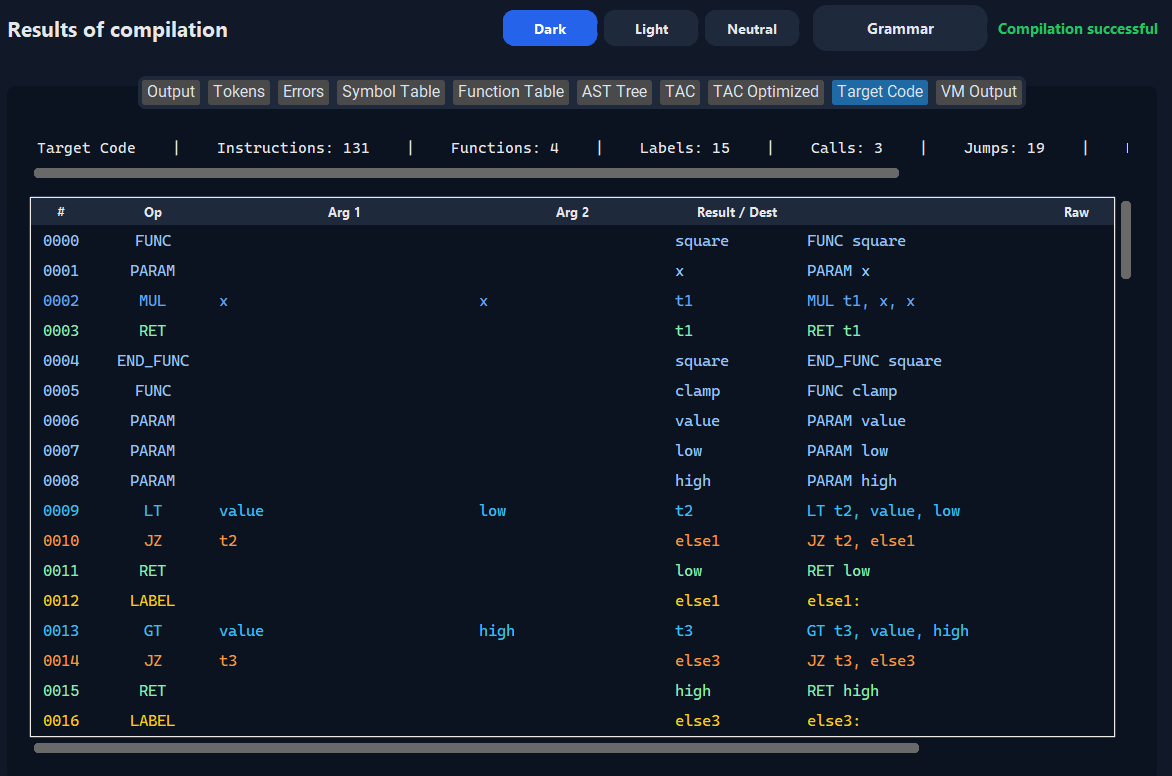
\includegraphics[width=\textwidth]{figs/test3_outputTarg.png}
		\caption{Target Code}
		\label{fig:test1_ast}
	\end{minipage}
    \hfill
	\begin{minipage}[t]{0.32\textwidth}
		\centering
		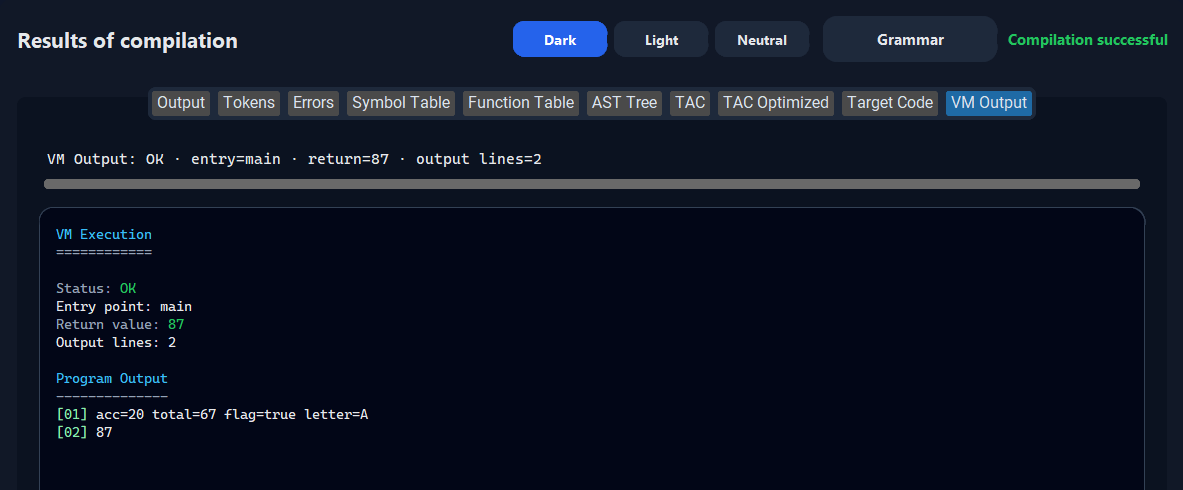
\includegraphics[width=\textwidth]{figs/test3_outputVM.png}
		\caption{VM Output}
		\label{fig:test1_ast}
	\end{minipage}
    
\end{figure}

\subsection{Invalid Test Cases}
\subsubsection{Test Case 4: Lexical Error (20\_lexical\_invalid\_symbol.c)}
Figure 34 shows the input source code containing a lexical error caused by the invalid character @, which does not belong to the language specification supported by the compiler. \\
Figure 35 presents the program output generated during the lexical analysis phase, where the compiler detects the invalid token and reports a lexical error message. \\
Finally, Figure 36 highlights the exact location in the source code where the lexical error occurred, allowing the user to identify and correct the invalid character.
\begin{figure}[H]
	\centering
	\begin{minipage}[t]{0.48\textwidth}
		\centering
		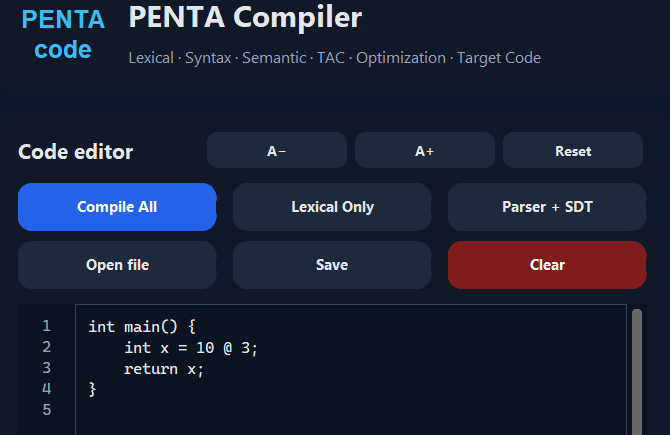
\includegraphics[width=\textwidth]{figs/test4_input.png}
		\caption{Input for Test Case 4}
		\label{fig:test1}
	\end{minipage}
	\hfill
	\begin{minipage}[t]{0.48\textwidth}
		\centering
		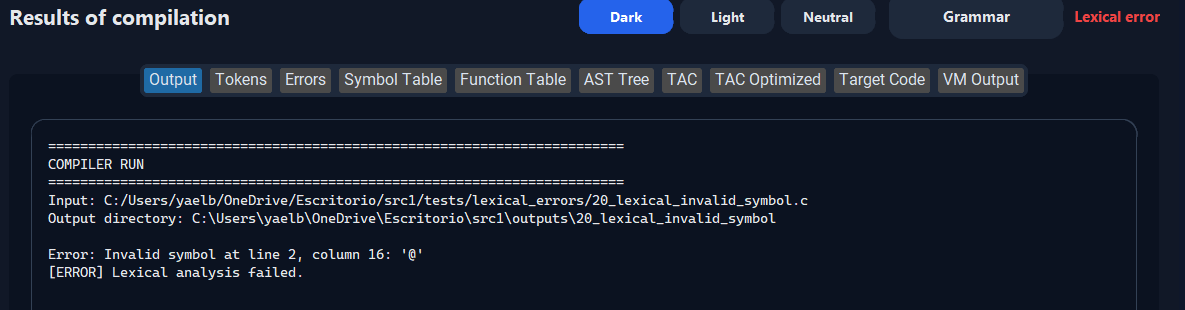
\includegraphics[width=\textwidth]{figs/test4_output.png}
		\caption{Output for Test Case 4}
		\label{fig:test1_ast}
	\end{minipage}
\end{figure}

\begin{figure}[H]
    \centering
	\begin{minipage}[t]{0.48\textwidth}
		\centering
		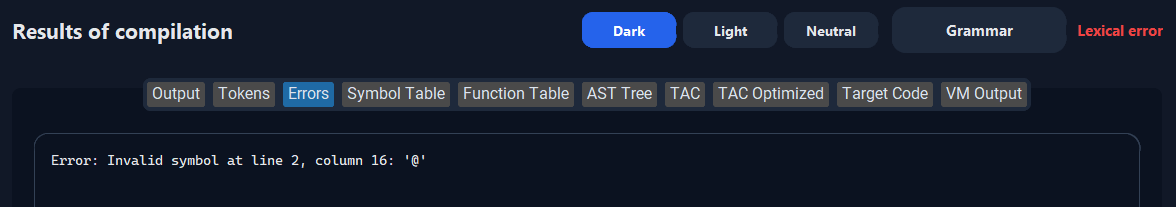
\includegraphics[width=\textwidth]{figs/test4_outputE.png}
		\caption{Errors}
		\label{fig:test1}
	\end{minipage}
\end{figure}


\subsubsection{Test Case 5: Sintax Error}
Figure 34 shows the input source code containing a syntax error caused by the missing semicolon after the variable assignment statement.
\\
Figure 35 presents the program output generated during the compilation process. The output indicates that the source code successfully passed the lexical analysis phase; however, the compilation process stopped during the syntax analysis phase due to a syntax error detected by the parser.
\\
Figure 36 displays the tokens and lexemes generated by the lexical analyzer before the syntax analysis process began. This confirms that the lexer correctly identified and classified the elements of the source code.
\\
Finally, Figure 37 highlights the exact location in the source code where the syntax error occurred, allowing the user to identify the missing semicolon and correct the statement.
\begin{figure}[H]
	\centering
	\begin{minipage}[t]{0.48\textwidth}
		\centering
		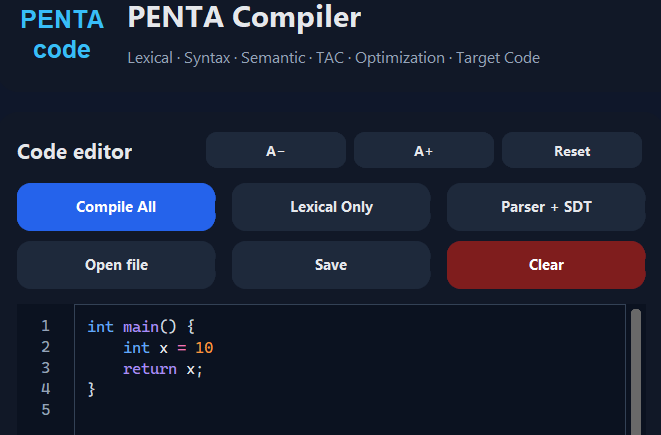
\includegraphics[width=\textwidth]{figs/test5_input.png}
		\caption{Input for Test Case 5}
		\label{fig:test1}
	\end{minipage}
	\hfill
	\begin{minipage}[t]{0.48\textwidth}
		\centering
		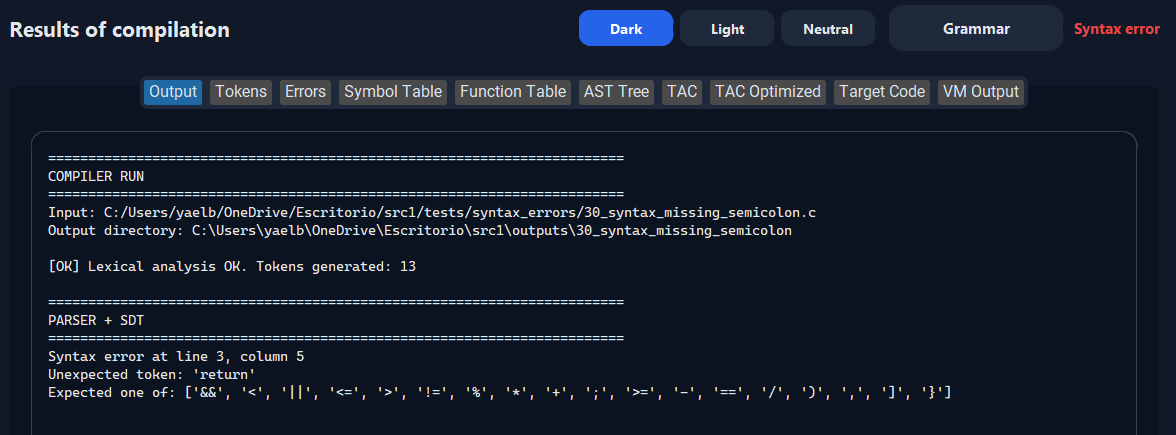
\includegraphics[width=\textwidth]{figs/test5_output.png}
		\caption{Output for Test Case 5}
		\label{fig:test1_ast}
	\end{minipage}    
\end{figure}

\begin{figure}[H]
    \begin{minipage}[t]{0.48\textwidth}
		\centering
		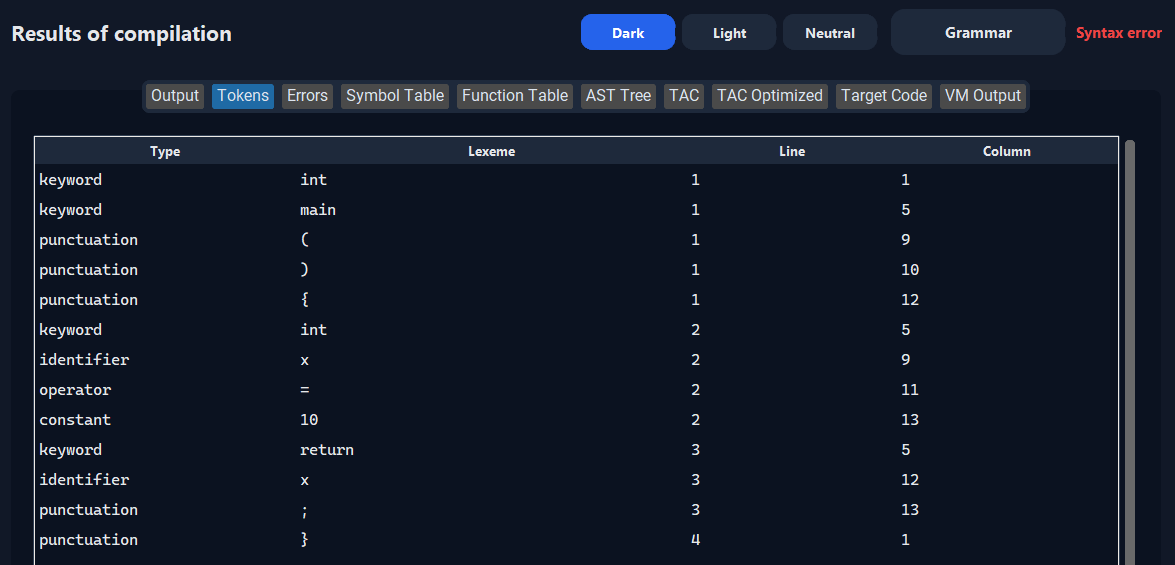
\includegraphics[width=\textwidth]{figs/test5_outputTok.png}
		\caption{Tokens}
		\label{fig:test1}
	\end{minipage}
	\hfill
	\begin{minipage}[t]{0.48\textwidth}
		\centering
		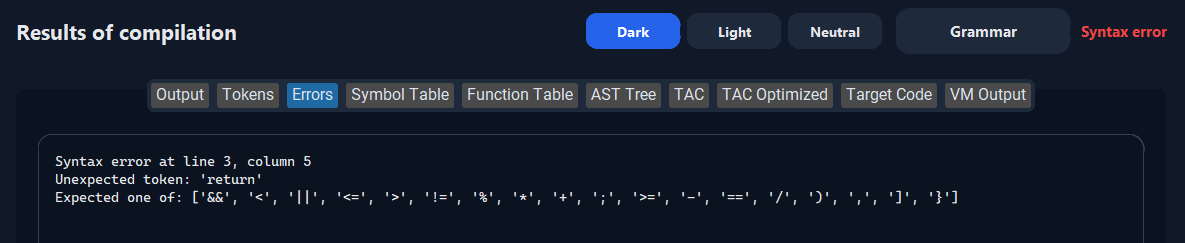
\includegraphics[width=\textwidth]{figs/test5_outputE.png}
		\caption{Errors}
		\label{fig:test1_ast}
	\end{minipage}
\end{figure}


\section{Conclusions}
The development of the compiler demonstrated how the theoretical foundations of compiler construction can be practically applied to solve the problem of validating and processing C source code. Through the integration of the different compilation phases, it was possible to establish a structured workflow capable of transforming high-level instructions into validated and executable internal representations.
\\
The obtained results highlight the importance of lexical analysis as the initial mechanism for token recognition and classification, since it provides an organized representation of the input that simplifies subsequent compiler stages. Likewise, syntax analysis based on LALR and Shift-Reduce techniques successfully validated the grammatical structure of programs, demonstrating the relevance of context-free grammars and LR automata in the construction of deterministic parsers.
\\
Furthermore, the incorporation of Syntax Directed Translation (SDT) confirmed the necessity of complementing syntactic validation with semantic verification. The implementation of symbol tables, abstract syntax trees, and semantic rules ensured logical consistency within the analyzed programs, detecting errors related to declarations, variable usage, and type consistency before execution.
\\
The valid and invalid test cases demonstrated that the system is capable of accurately identifying and classifying lexical, syntactic, and semantic errors. In addition, the generation of intermediate representations, optimized code, and target code showed the relationship between theoretical compilation phases and their practical implementation within a functional compiler architecture.
\\
Overall, the project demonstrates that the integrated application of concepts such as regular expressions, context-free grammars, LR/LALR parsing, SDT, and semantic structures constitutes an effective solution for modern compiler design, validating the importance of these foundations within the field in which we operate.
\printbibliography
\end{document}
